
%% bare_conf.tex
%% V1.3
%% 2007/01/11
%% by Michael Shell
%% See:
%% http://www.michaelshell.org/
%% for current contact information.
%%
%% This is a skeleton file demonstrating the use of IEEEtran.cls
%% (requires IEEEtran.cls version 1.7 or later) with an IEEE conference paper.
%%
%% Support sites:
%% http://www.michaelshell.org/tex/ieeetran/
%% http://www.ctan.org/tex-archive/macros/latex/contrib/IEEEtran/
%% and
%% http://www.ieee.org/

%%*************************************************************************
%% Legal Notice:
%% This code is offered as-is without any warranty either expressed or
%% implied; without even the implied warranty of MERCHANTABILITY or
%% FITNESS FOR A PARTICULAR PURPOSE! 
%% User assumes all risk.
%% In no event shall IEEE or any contributor to this code be liable for
%% any damages or losses, including, but not limited to, incidental,
%% consequential, or any other damages, resulting from the use or misuse
%% of any information contained here.
%%
%% All comments are the opinions of their respective authors and are not
%% necessarily endorsed by the IEEE.
%%
%% This work is distributed under the LaTeX Project Public License (LPPL)
%% ( http://www.latex-project.org/ ) version 1.3, and may be freely used,
%% distributed and modified. A copy of the LPPL, version 1.3, is included
%% in the base LaTeX documentation of all distributions of LaTeX released
%% 2003/12/01 or later.
%% Retain all contribution notices and credits.
%% ** Modified files should be clearly indicated as such, including  **
%% ** renaming them and changing author support contact information. **
%%
%% File list of work: IEEEtran.cls, IEEEtran_HOWTO.pdf, bare_adv.tex,
%%                    bare_conf.tex, bare_jrnl.tex, bare_jrnl_compsoc.tex
%%*************************************************************************

% *** Authors should verify (and, if needed, correct) their LaTeX system  ***
% *** with the testflow diagnostic prior to trusting their LaTeX platform ***
% *** with production work. IEEE's font choices can trigger bugs that do  ***
% *** not appear when using other class files.                            ***
% The testflow support page is at:
% http://www.michaelshell.org/tex/testflow/



% Note that the a4paper option is mainly intended so that authors in
% countries using A4 can easily print to A4 and see how their papers will
% look in print - the typesetting of the document will not typically be
% affected with changes in paper size (but the bottom and side margins will).
% Use the testflow package mentioned above to verify correct handling of
% both paper sizes by the user's LaTeX system.
%
% Also note that the "draftcls" or "draftclsnofoot", not "draft", option
% should be used if it is desired that the figures are to be displayed in
% draft mode.
%
\documentclass[conference]{IEEEtran}
% Add the compsoc option for Computer Society conferences.
%
% If IEEEtran.cls has not been installed into the LaTeX system files,
% manually specify the path to it like:
% \documentclass[conference]{../sty/IEEEtran}
\usepackage[utf8]{inputenc}
\usepackage[spanish]{babel}


% Some very useful LaTeX packages include:
% (uncomment the ones you want to load)


% *** MISC UTILITY PACKAGES ***
%
%\usepackage{ifpdf}
% Heiko Oberdiek's ifpdf.sty is very useful if you need conditional
% compilation based on whether the output is pdf or dvi.
% usage:
% \ifpdf
%   % pdf code
% \else
%   % dvi code
% \fi
% The latest version of ifpdf.sty can be obtained from:
% http://www.ctan.org/tex-archive/macros/latex/contrib/oberdiek/
% Also, note that IEEEtran.cls V1.7 and later provides a builtin
% \ifCLASSINFOpdf conditional that works the same way.
% When switching from latex to pdflatex and vice-versa, the compiler may
% have to be run twice to clear warning/error messages.






% *** CITATION PACKAGES ***
%
%\usepackage{cite}
%%\usepackage{bibtex}
%\bibliographystyle{IEEEtran}
%\bibliography{IEEEabrv,BiblioTh7}
% cite.sty was written by Donald Arseneau
% V1.6 and later of IEEEtran pre-defines the format of the cite.sty package
% \cite{} output to follow that of IEEE. Loading the cite package will
% result in citation numbers being automatically sorted and properly
% "compressed/ranged". e.g., [1], [9], [2], [7], [5], [6] without using
% cite.sty will become [1], [2], [5]--[7], [9] using cite.sty. cite.sty's
% \cite will automatically add leading space, if needed. Use cite.sty's
% noadjust option (cite.sty V3.8 and later) if you want to turn this off.
% cite.sty is already installed on most LaTeX systems. Be sure and use
% version 4.0 (2003-05-27) and later if using hyperref.sty. cite.sty does
% not currently provide for hyperlinked citations.
% The latest version can be obtained at:
% http://www.ctan.org/tex-archive/macros/latex/contrib/cite/
% The documentation is contained in the cite.sty file itself.






% *** GRAPHICS RELATED PACKAGES ***
%
\ifCLASSINFOpdf
   \usepackage[pdftex]{graphicx}
  % declare the path(s) where your graphic files are
  % \graphicspath{{../pdf/}{../jpeg/}}
  % and their extensions so you won't have to specify these with
  % every instance of \includegraphics
  % \DeclareGraphicsExtensions{.pdf,.jpeg,.png}
\else
  % or other class option (dvipsone, dvipdf, if not using dvips). graphicx
  % will default to the driver specified in the system graphics.cfg if no
  % driver is specified.
   \usepackage[dvips]{graphicx}
  % declare the path(s) where your graphic files are
  % \graphicspath{{../eps/}}
  % and their extensions so you won't have to specify these with
  % every instance of \includegraphics
  % \DeclareGraphicsExtensions{.eps}
\fi
% graphicx was written by David Carlisle and Sebastian Rahtz. It is
% required if you want graphics, photos, etc. graphicx.sty is already
% installed on most LaTeX systems. The latest version and documentation can
% be obtained at: 
% http://www.ctan.org/tex-archive/macros/latex/required/graphics/
% Another good source of documentation is "Using Imported Graphics in
% LaTeX2e" by Keith Reckdahl which can be found as epslatex.ps or
% epslatex.pdf at: http://www.ctan.org/tex-archive/info/
%
% latex, and pdflatex in dvi mode, support graphics in encapsulated
% postscript (.eps) format. pdflatex in pdf mode supports graphics
% in .pdf, .jpeg, .png and .mps (metapost) formats. Users should ensure
% that all non-photo figures use a vector format (.eps, .pdf, .mps) and
% not a bitmapped formats (.jpeg, .png). IEEE frowns on bitmapped formats
% which can result in "jaggedy"/blurry rendering of lines and letters as
% well as large increases in file sizes.
%
% You can find documentation about the pdfTeX application at:
% http://www.tug.org/applications/pdftex





% *** MATH PACKAGES ***
%
\usepackage[cmex10]{amsmath}
\usepackage{amssymb}
\usepackage{marvosym}
% A popular package from the American Mathematical Society that provides
% many useful and powerful commands for dealing with mathematics. If using
% it, be sure to load this package with the cmex10 option to ensure that
% only type 1 fonts will utilized at all point sizes. Without this option,
% it is possible that some math symbols, particularly those within
% footnotes, will be rendered in bitmap form which will result in a
% document that can not be IEEE Xplore compliant!
%
% Also, note that the amsmath package sets \interdisplaylinepenalty to 10000
% thus preventing page breaks from occurring within multiline equations. Use:
\interdisplaylinepenalty=2500
% after loading amsmath to restore such page breaks as IEEEtran.cls normally
% does. amsmath.sty is already installed on most LaTeX systems. The latest
% version and documentation can be obtained at:
% http://www.ctan.org/tex-archive/macros/latex/required/amslatex/math/




% *** SPECIALIZED LIST PACKAGES ***
%
%\usepackage{algorithmic}
% algorithmic.sty was written by Peter Williams and Rogerio Brito.
% This package provides an algorithmic environment fo describing algorithms.
% You can use the algorithmic environment in-text or within a figure
% environment to provide for a floating algorithm. Do NOT use the algorithm
% floating environment provided by algorithm.sty (by the same authors) or
% algorithm2e.sty (by Christophe Fiorio) as IEEE does not use dedicated
% algorithm float types and packages that provide these will not provide
% correct IEEE style captions. The latest version and documentation of
% algorithmic.sty can be obtained at:
% http://www.ctan.org/tex-archive/macros/latex/contrib/algorithms/
% There is also a support site at:
% http://algorithms.berlios.de/index.html
% Also of interest may be the (relatively newer and more customizable)
% algorithmicx.sty package by Szasz Janos:
% http://www.ctan.org/tex-archive/macros/latex/contrib/algorithmicx/




% *** ALIGNMENT PACKAGES ***
%
%\usepackage{array}
% Frank Mittelbach's and David Carlisle's array.sty patches and improves
% the standard LaTeX2e array and tabular environments to provide better
% appearance and additional user controls. As the default LaTeX2e table
% generation code is lacking to the point of almost being broken with
% respect to the quality of the end results, all users are strongly
% advised to use an enhanced (at the very least that provided by array.sty)
% set of table tools. array.sty is already installed on most systems. The
% latest version and documentation can be obtained at:
% http://www.ctan.org/tex-archive/macros/latex/required/tools/


%\usepackage{mdwmath}
%\usepackage{mdwtab}
% Also highly recommended is Mark Wooding's extremely powerful MDW tools,
% especially mdwmath.sty and mdwtab.sty which are used to format equations
% and tables, respectively. The MDWtools set is already installed on most
% LaTeX systems. The lastest version and documentation is available at:
% http://www.ctan.org/tex-archive/macros/latex/contrib/mdwtools/


% IEEEtran contains the IEEEeqnarray family of commands that can be used to
% generate multiline equations as well as matrices, tables, etc., of high
% quality.


%\usepackage{eqparbox}
% Also of notable interest is Scott Pakin's eqparbox package for creating
% (automatically sized) equal width boxes - aka "natural width parboxes".
% Available at:
% http://www.ctan.org/tex-archive/macros/latex/contrib/eqparbox/





% *** SUBFIGURE PACKAGES ***
%\usepackage[tight,footnotesize]{subfigure}
% subfigure.sty was written by Steven Douglas Cochran. This package makes it
% easy to put subfigures in your figures. e.g., "Figure 1a and 1b". For IEEE
% work, it is a good idea to load it with the tight package option to reduce
% the amount of white space around the subfigures. subfigure.sty is already
% installed on most LaTeX systems. The latest version and documentation can
% be obtained at:
% http://www.ctan.org/tex-archive/obsolete/macros/latex/contrib/subfigure/
% subfigure.sty has been superceeded by subfig.sty.



%\usepackage[caption=false]{caption}
%\usepackage[font=footnotesize]{subfig}
% subfig.sty, also written by Steven Douglas Cochran, is the modern
% replacement for subfigure.sty. However, subfig.sty requires and
% automatically loads Axel Sommerfeldt's caption.sty which will override
% IEEEtran.cls handling of captions and this will result in nonIEEE style
% figure/table captions. To prevent this problem, be sure and preload
% caption.sty with its "caption=false" package option. This is will preserve
% IEEEtran.cls handing of captions. Version 1.3 (2005/06/28) and later 
% (recommended due to many improvements over 1.2) of subfig.sty supports
% the caption=false option directly:
%\usepackage[caption=false,font=footnotesize]{subfig}
%
% The latest version and documentation can be obtained at:
% http://www.ctan.org/tex-archive/macros/latex/contrib/subfig/
% The latest version and documentation of caption.sty can be obtained at:
% http://www.ctan.org/tex-archive/macros/latex/contrib/caption/




% *** FLOAT PACKAGES ***
%
%\usepackage{fixltx2e}
% fixltx2e, the successor to the earlier fix2col.sty, was written by
% Frank Mittelbach and David Carlisle. This package corrects a few problems
% in the LaTeX2e kernel, the most notable of which is that in current
% LaTeX2e releases, the ordering of single and double column floats is not
% guaranteed to be preserved. Thus, an unpatched LaTeX2e can allow a
% single column figure to be placed prior to an earlier double column
% figure. The latest version and documentation can be found at:
% http://www.ctan.org/tex-archive/macros/latex/base/



%\usepackage{stfloats}
% stfloats.sty was written by Sigitas Tolusis. This package gives LaTeX2e
% the ability to do double column floats at the bottom of the page as well
% as the top. (e.g., "\begin{figure*}[!b]" is not normally possible in
% LaTeX2e). It also provides a command:
%\fnbelowfloat
% to enable the placement of footnotes below bottom floats (the standard
% LaTeX2e kernel puts them above bottom floats). This is an invasive package
% which rewrites many portions of the LaTeX2e float routines. It may not work
% with other packages that modify the LaTeX2e float routines. The latest
% version and documentation can be obtained at:
% http://www.ctan.org/tex-archive/macros/latex/contrib/sttools/
% Documentation is contained in the stfloats.sty comments as well as in the
% presfull.pdf file. Do not use the stfloats baselinefloat ability as IEEE
% does not allow \baselineskip to stretch. Authors submitting work to the
% IEEE should note that IEEE rarely uses double column equations and
% that authors should try to avoid such use. Do not be tempted to use the
% cuted.sty or midfloat.sty packages (also by Sigitas Tolusis) as IEEE does
% not format its papers in such ways.





% *** PDF, URL AND HYPERLINK PACKAGES ***
%
%\usepackage{url}
% url.sty was written by Donald Arseneau. It provides better support for
% handling and breaking URLs. url.sty is already installed on most LaTeX
% systems. The latest version can be obtained at:
% http://www.ctan.org/tex-archive/macros/latex/contrib/misc/
% Read the url.sty source comments for usage information. Basically,
% \url{my_url_here}.





% *** Do not adjust lengths that control margins, column widths, etc. ***
% *** Do not use packages that alter fonts (such as pslatex).         ***
% There should be no need to do such things with IEEEtran.cls V1.6 and later.
% (Unless specifically asked to do so by the journal or conference you plan
% to submit to, of course. )


% correct bad hyphenation here
\hyphenation{op-tical net-works semi-conduc-tor}
%my macros
\newcommand{\marco}[1]{\{\mathcal{#1}\}}
\DeclareMathOperator{\sinc}{sinc}
\newtheorem {defin}{Definición}[section]
\newcommand{\parderiv}[2]{\frac{\partial #1}{\partial #2}}
\begin{document}
%
% paper title
% can use linebreaks \\ within to get better formatting as desired
\title{Evaluación experimental de la Reconstrucción en cuaterniones de la Matriz de Rotación con un Observador Óptimo/EKF en un Algoritmo de Navegación de Observadores en Cascada del Tipo Filtro Complementario en SO(3)}

% author names and affiliations
% use a multiple column layout for up to three different
% affiliations
%\author{\IEEEauthorblockN{Ariel Iporre R.}
%\IEEEauthorblockA{Universidad Mayor de San Andrés\\
%Facultad de Ingeniería\\
%Ingenieria Electrónica\\
%La Paz, Bolivia\\
%Email: aiporre@umsa.bo}
%\and
%\IEEEauthorblockN{Mauricio Améstegui}
%\IEEEauthorblockA{Universidad Mayor de San Andrés\\
%Facultad de Ingeniería\\
%Ingenieria Electrónica\\
%La Paz, Bolivia\\
%Email: mamestegui@umsa.bo}
%}

% conference papers do not typically use \thanks and this command
% is locked out in conference mode. If really needed, such as for
% the acknowledgment of grants, issue a \IEEEoverridecommandlockouts
% after \documentclass

% for over three affiliations, or if they all won't fit within the width
% of the page, use this alternative format:
% 
\author{\IEEEauthorblockN{Autor 1.\IEEEauthorrefmark{1} y
Autor 2.\IEEEauthorrefmark{1}}
\IEEEauthorblockA{\IEEEauthorrefmark{1}Ingeniería Electrónica-Facultad de Ingeniería\\Universidad Mayor de San Andrés,
La Paz, Bolivia\\ Email: aiporre@umsa.bo, mamestegui@umsa.bo}}




% use for special paper notices
%\IEEEspecialpapernotice{(Invited Paper)}




% make the title area
\maketitle
\textbf{\small \emph{Abstract}--This work proposed a variation for a erlier navigation algorithm in the literature composed by SO(3) complementary filters. Such modification determines the inclution of a quaternion optimal observer to determine  the rotation matrix instead using a vectorial reconstruction approach, that proposal involves an experimental comparison between the original and modified method. The results show a 40\% increase for estimation quality while 21\% more complexity using this new approach. It also verifies the implementation in real noise environment.\\[3mm]}
\begin{abstract}
%\boldmath
Este trabajo propone la variación de un algoritmo compuesto por Filtros Complementarios en el Espacio Ortogonal Especial de la literatura. La variación incorpora un Observador Óptimo EKF en cuaterniones para la determinación de la matriz de rotación de forma óptima en lugar de calcularla de forma directa en base al punto de estabilidad de los filtros. Está modificación implicó la comparación experimental entre el método original y el método modificado; los resultados de tal comparación muestran hasta un 40\% de mejora en la calidad de la estimación, frente a 21\% más de tiempo de procesamiento o latencia de cálculo. Asimismo, los experimentos en condiciones reales comprueban la factibilidad de la implementación del algoritmo en condiciones adversas de ruido e incertidumbre de medición.\end{abstract}
% IEEEtran.cls defaults to using nonbold math in the Abstract.
% This preserves the distinction between vectors and scalars. However,
% if the conference you are submitting to favors bold math in the abstract,
% then you can use LaTeX's standard command \boldmath at the very start
% of the abstract to achieve this. Many IEEE journals/conferences frown on
% math in the abstract anyway.

% no keywords




% For peer review papers, you can put extra information on the cover
% page as needed:
% \ifCLASSOPTIONpeerreview
% \begin{center} \bfseries EDICS Category: 3-BBND \end{center}
% \fi
%
% For peerreview papers, this IEEEtran command inserts a page break and
% creates the second title. It will be ignored for other modes.
\IEEEpeerreviewmaketitle



\section{Introducción}
A medida que los sensores de navegación y los procesadores computacionales reducían su tamaño, los algoritmos de navegación debieron especializarse progresivamente en la búsqueda de una mejor precisión en la estimación de los estados de navegación. En esa línea, durante la década de los 60's, el desarrollo del Filtro Schmidt-Kalman \cite{Schmidt1966} o más conocido como el Filtro de Kalman Extendido (EKF) incorpora los conceptos de estimación y observación de la teoría de control en la tecnología de los sistemas de navegación; este abordaje propone la aplicación del Filtro de Kalman \cite{Kalman1960} en un sistema no lineal para la resolución del problema de navegación, definido en la referencia \cite{Schmidt1962}. De ahí en adelante, varios autores desarrollan una gran cantidad de técnicas, e.g. filtro de Kalman extendido (EKF), algoritmos genéticos, redes neuronales, filtros de partículas o el algoritmo QUEST.\par
En la década de los noventa los algoritmos de navegación fueron constituidos por observadores no lineales desarrollados en el marco de la teoría de Lyapunov, %Aquí hay un hueco en revisión de los artículos menciodosx
evidenciable en los trabajos \cite{Lukyanov1996,Nicosia1996,Algrain1997}. De donde deriva el énfasis de investigación de algoritmos de navegación alrededor de esta temática, se centra en la extensión de estas técnicas para la determinación de posición incorporando sensores basados en el \emph{Sistema de Posicionamiento Global} (GPS), o cámaras Web.\par
%%
De esa manera, los algoritmos de navegación modernos están siempre concretados en una técnica de estimación, y dependiendo de la aplicación diferentes sensores de navegación son usados. Y cuando el movimiento abarca grandes áreas, los sensores deben ser de muy buena calidad, o medir parámetros absolutos, como es el caso del GPS, la triangulación por medio del sistema global para comunicaciones móviles (Global System for Mobile Communications ó originalmente Groupe Spécial Mobile, GSM), o el GPS asistido (AGPS).\par
%%Revisión y discusión de trabajos previos
El EKF, usado en este trabajo para la determinación de la matriz de rotación, es celebrado como uno de los enfoques de filtros estadísticos de mayor éxito y que actualmente tiene un rango de desarrollo increíblemente amplio. Este algoritmo es prácticamente el algoritmo de navegación por excelencia e indudablemente la técnica más utilizada en los sistemas de navegación; esto es demostrable en la extensa lista de trabajos en variedades del Filtro de Kalman enfocado a esta temática que se pueden encontrar en la literatura, e.g.\cite{Faruki2000, Marins2001, Gandhi2007, Sabatini2006, Bistrovs2012}. Dentro de las varias representaciones del EKF implementadas, priman las denominadas EKF multiplicativo (MEKF), los cuales mantienen la estructura general EKF, pero son desarrollados alrededor de un modelo de error \cite{Friedland1978,Benson1975}.\par
%%
El EKF guarda una estrecha relación con el observador óptimo del esquema de Luenberger. Y particularmente, se han concretado algunos Filtros de Kalman desde la teoría del control óptimo para la estimación de la información de navegación \cite{Smith1995}.\par
%
El limitado, pero novedoso método de \cite{Kou1975} y \cite{Thau1973} para el diseño de un observador no lineal como una extensión del observador de Luenberger, ha abierto un nueva brecha en metodologías para la determinación de la información de navegación. Lo anteriormente mencionado se constata en las referencias: \cite{Vik2001,Thienel2003} y \cite{Hua2009}, los cuales aplican los conceptos de la teoría de Lyapunov en el diseño de varios observadores que calculan la información de navegación.\par
%%
Este tipo de enfoque basa su análisis en la búsqueda de la condición de estabilidad en el sentido de Lyapunov. De manera similar, los filtros complementarios en un Grupo Ortogonal Especial $SO(3)$\footnote{Un Grupo Ortogonal Especial está constituido por un grupo de matrices de transformación que hacen rotaciones propias a los elementos de Espacio Euclídeo.} de \cite{Mahony2008} y \cite{Scandaro2011}, definen las constantes de actualización en un grupo ortogonal especial a partir de funciones de Lyapunov; o los observadores invariantes como \cite{Bonabel2008} y \cite{Martin2008}; los cuales mantienen una simetría utilizando mediciones auxiliares del mismo parámetro que se estima. %FALTA LEER OBSERVADORES INVARIANTES!!! NO ESTA CLARO
\par
%
También, se han hecho esfuerzos por combinar diferentes tipos de observadores, por ejemplo: en \cite{Vasconcelos2008} se presenta una configuración de dos observadores en cascada para la estimación de la matriz de rotación y la estimación de la posición, donde los observadores son diseñados usando el análisis de estabilidad de Lyapunov; o en \cite{Scandaro2011} que también combina dos observadores en cascada para la determinación de la orientación y la posición, con ambos observadores con una configuración especial parecida al filtro complementario en frecuencia.\footnote{Donde, el observador de orientación es el usado en \cite{Mahony2008}. }. A partir de esto, la idea en este trabajo es el establecimiento de un \emph{algoritmo de navegación} compuesto de una serie de \emph{observadores de estado}, que busca una mejora de la estimación de la información de navegación.\par
De manera general, existen dos puntos importantes que se abordan en el desarrollo de este proyecto:
\begin{itemize}
\item El primero es la modificación del \emph{algoritmo de observadores no lineales tipo filtro complementario en un grupo ortogonal especial SO(3) de Mahony y Scandaroli} (desarrollado por estos dos autores en las referencias \cite{Mahony2008,Scandaro2011}) con la inclusión de un observador óptimo tipo Filtro de Kalman Extendido (EKF)\footnote{El filtro de Kalman, fue desarrollado Rudolf Kalman en [\cite{Kalman1960}]} para la determinación de la matriz de rotación.
\item Como segundo punto se tiene el desarrollo de una serie de experimentos que establecen la evaluación experimental para comprobar una mejora del algoritmo modificado con respecto al algoritmo original. \end{itemize}\par
%%%%%%%%%%%%%%%
%%%%%%%%%%%%%%%
\section{Problema de navegación: Algoritmo de navegación de Mahony-Scandarolli}
%%%%%%%%%%%%%%%
%%%%%%%%%%%%%%%
La solución al problema de navegación se delimita en la determinación dos las condiciones que describen el movimiento de un cuerpo (Información de Navegación): la situación espacial (¿dónde estoy?); y el ritmo de cambio de cambio de dicha situación (¿hacia dónde voy?), es decir rumbo o vector de velocidad. Es así que con el afán de determinar dichas condiciones, el algoritmo de navegación, dentro del sistema de navegación, interpreta la medición de parámetros del medio o que son consecuencia del propio movimiento, para recuperar las variables que describen: tanto la situación espacial como su ritmo de cambio; o dicho de otra manera reconstruye la información de navegación\footnote{Variables que describen el movimiento} a partir de información corrompida y parcial relacionada con las variables del movimiento, que es proporcionada por sensores de navegación.\par
%%
Tomando en cuenta esto, el problema de navegación se traduce en el reto del planteamiento de un algoritmo de navegación, es decir contruir la secuencia de operaciónes para determinación la información de navegación\footnote{En el presente trabajo, el conjunto de variables, compuestas por: la velocidad lineal, velocidad angular, posición y orientación, es denominado \emph{información de navegación}. Este describe el movimiento de un cuerpo rígido de seis grados libertad.}($X$), a partir del conjunto, denominado \emph{información sensorial disponible} ($S$), que se compone de las mediciones obtenidas de sensores de navegación\par
\begin{figure}
\begin{center}
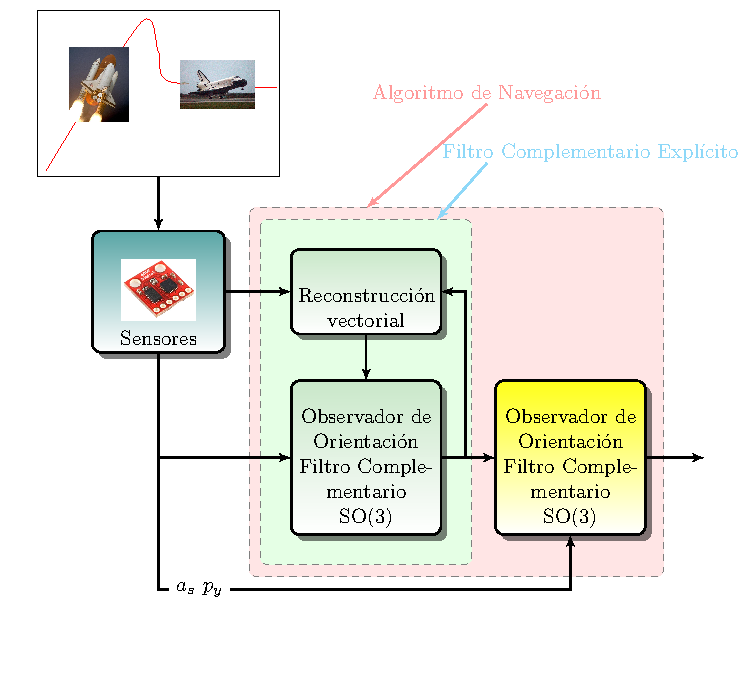
\includegraphics[width=9cm,clip]{intro_fig4.pdf}
\caption{Esquema simplificado del algoritmo de Mahony-Scandaroli.}
\scriptsize{Tell us about.}
\label{solucionMS_fig1}
\end{center}
\end{figure}
La solución de este problema, desde el enfoque de Mahony-Scandaroli, deriva en el algoritmo de navegación de filtros complementarios en SO(3) en cascada, esquematizado en diagrama de bloques de la Figura \ref{solucionMS_fig1}. Este propone la combinación en cascada de dos observadores del tipo filtro complementario en SO(3), el observador de orientación y el observador de posición; en donde el observador orientación utiliza la medición de la velocidad angular $\Omega_s$ \footnote{ Elemento de conjunto de \emph{información sensorial disponible} $S$} y la matriz de rotación $R_y$ proveniente de una fórmula de  reconstrucción vectorial,  que conjuga: la medición de valores vectoriales en $\marco{B}$ ($v_i$), sus valores teóricos en el $\marco{A}$ ($v_{i,0}$), y el punto de estabilidad encontrado por el observador de orientación para la matriz de rotación ($\hat{R}$, estos relacionados en la siguiente ecuación, en la que se toma en cuenta $n$ mediciones vectoriales.
\begin{equation}\label{ReconstruccionVectorial}
R_y=\sum_{i=1}^{n}(v_{i,0})_\times\hat{R}(v_i)_\times
\end{equation}
%%%%%
El observador de orientación toma estas variables para la determinación de: 
\begin{itemize}
\item $\hat{\Theta}$: La orientación en términos de los ángulos de Euler .
\item  $\hat{\Omega}$: La velocidad angular en $\marco{B}$, donde $\marco{B}$ denota un marco referencial cartesiano fijo al cuerpo desde donde se realiza la medición de la aceleración y velocidad angular.
\item $\tilde{R}$: El error de estimación de la matriz de rotación, definida a través de la matriz de transformación $\marco{E}\hookrightarrow\marco{B}$, donde $\marco{E}$ denota el marco referencial de estimación, el cual teóricamente converge hacia $\marco{B}$ y se considera el resultado de la estimación de $\marco{B}$ por el observador de orientación .
\item $\hat{R}$: La estimación de la matriz de rotación, definida como la matriz de transformación $ \marco{E}\hookrightarrow\marco{A}$,  donde $\marco{A}$ denota el marco referencial inercial, con direccion y origen fijos en un punto sobre la tierra.
\end{itemize}
Siguiendo este esquema del algoritmo de navegación de Mahony-Scandarolli, en cascada el observador de posición tipo Filtro complementario en SO(3), toma el resto de las variables incluidas en $S$ (la medición de la aceleración $a_s$ y la medición de la posición $p_y$), junto con las matrices de transformación determinadas por el anterior observador, para obtener:
\begin{itemize}
\item $\hat{p}$: La estimación de la posición en $\marco{A}$.
\item $\hat{v}$: La estimación de la velocidad en $\marco{A}$.
\end{itemize}
Finalmente, los dos grupos de variables estimadas por ambos observadores conforman la \emph{estimación de la información de navegación}, que puede ser denotada por el vector columna $X=[\hat{p}~\hat{v}~\hat{\Theta}~\hat{\Omega}]$.\par

%En resumen, el enfoque original del algoritmo de observadores en cascada de Mahony-Scandaroli, resuelve la determinación de la información de navegación en tres niveles de procesamiento:
%a) la reconstrucción vectorial de la matriz de rotación $R_y$ usando la medición de un acelerómetro $a_s$ y un magnetómetro $m_s$\footnote{El desarrollo teórico y práctico de Mahony en \cite{Mahony2008} demuestra que no es absolutamente necesario incluir ambas mediciones. Y si el caso fuese de que alguna de las señales es demasiado ruidosa se puede prescindir de la misma.}; b) la determinación de la estimación de la velocidad angular $\hat{\Omega}$, la estimación de la orientación en términos de los ángulos de Euler $\hat{\Theta}$, y la estimación de la matriz de rotación $\hat{R}$ con su respectivo error $\tilde{R}$\footnote{Definida como $\tilde{R}=R_y\hat{R}^T$}, los que se determinan usando las señales de la reconstrucción vectorial y la medición de un giroscopio $\Omega_s$; c) la determinación de la estimación de la posición $\hat{p}$, y la velocidad lineal $\hat{v}$ a partir de las anteriores salidas, es decir $\tilde{R}$ y $\hat{R}$, junto con la medición de posición $p_y$ y la aceleración $a_s$.\par
%%
Como señala Mahony, la principal desventaja en la formulación de los filtros complementarios pasivo y directo es la sensibilidad a la matriz de entrada $R_y$. Esta matriz es usada en el mapeo de la medición de la velocidad angular al marco inercial $\marco{A}$, y por esta razón, la determinación de esta matriz juega un papel central en el desempeño final del sistema. Considerando esto la determinación desde el enfoque de la reconstrucción vectorial del Mahony-Scandarolli, la recontrución sub-óptima basada en la resolucción de la ecuación de Lyapunov incorpora una sensibilidad extra: a ruidos de medición, sesgos de medición y los estados transitorios de ascentamiento. Esto último consolida relaciones no lineales de alto orden (ver ecuación \ref{ReconstruccionVectorial}) en el lazo de realimentación y el sistema dinámico del error de estimación estimación.\par

%%%%%%%%%%%%%%
%%%%%%%%%%%%%%
%%%%%%%%%%%%%%
\section{Reconstrucción Óptima de la matriz de rotación}
%%
Considerando las desventajas señaladas en la sección anterior, se indentifica que el mejorar la reconstrucción de la matriz de rotación puede traer mejoras en en el desempeño general del algoritmo. Para ello, se buscará solucionar de manera óptima el problema de determinación de la matriz de rotación\footnote{Planteado en la referencia \cite{Mahony2008}} a partir de mediciones vectoriales, el cual indica que: \emph{a partir de la medición de cantidades vectoriales conocidas respecto a $\marco{B}$, la matriz de rotación puede ser determinada en el argumento que minimiza la función de coste definida como:}
\begin{equation}\label{ProblemaOptimizacion}
R^*=\arg~\min_{R}\left\{\sum_i|v_{0,i}-Rv_{m,i}|^2\right\}
\end{equation}
Donde, la matriz de rotación óptima $R^*$ es obtenida en el argumento que minimiza la función de coste compuesta por la suma de los cuadrados de los módulos de la diferencia de: los valores de las mediciones vectoriales rotadas al marco inercial (R$v_{m,i}$), respecto a los valores teóricos conocidos de dichas cantidades vectoriales ($v_{0,i}$)\footnote{Donde los sub-índices corresponden a las distintos valores vectoriales medibles.}
%%%%%%%%%%%%%%
%%%%%%%%%%%%%%
%%%%%%%%%%%%%%
\subsection{Determinación óptima de la matriz de rotación a partir del modelo de medición del vector gravitacional en cuaterniones.}
\begin{figure} [t]
\begin{center}
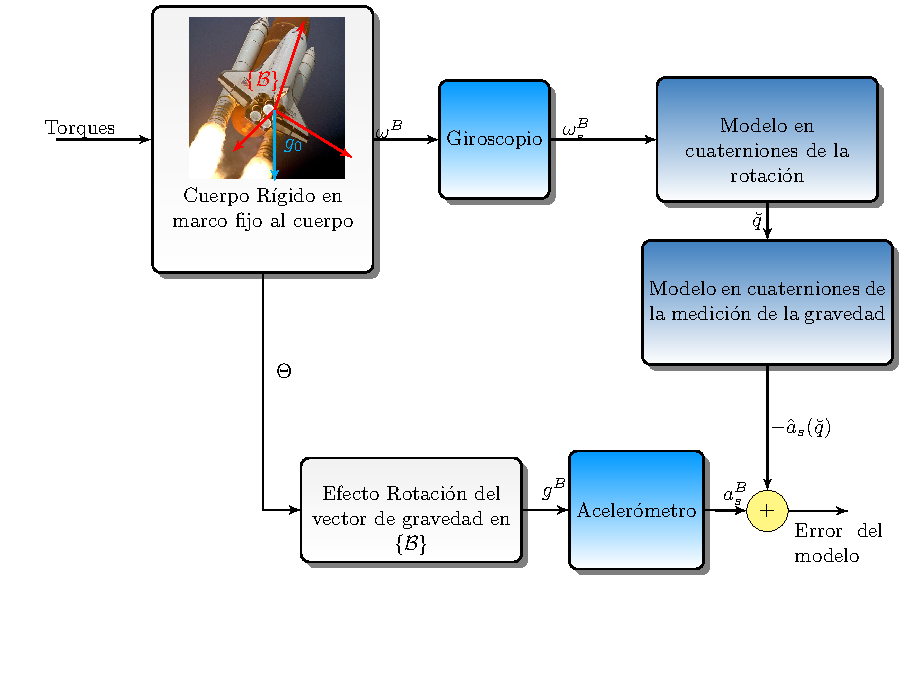
\includegraphics[scale=0.50,viewport=20 50 430 330,clip]{ObsOptimo_fig3.pdf}
\caption{Caracterización del error del modelo de medición.}
\label{ObsOptimo_fig2}
\end{center}
\end{figure}
%%
Se propone la determinación de la matriz de rotación interpretando el fenómeno de inclinación de campo gravitacional respecto al marco $\marco{B}$ con un observador óptimo en cuaterniones. Para ello, se identifica el cuaternión unitario\footnote{Los cuaterniones son una generalización de los números complejos en cuatro dimensiones, introducidas por Hamilton en 1853. El lector interesado en un desarrollo histórico de la teoría en cuaterniones, ver referencia [\cite{Warden1976}]}  en la relación que establece el problema de optimización de la matriz de rotación: 
\begin{equation}\label{ProblemaOptimizacionAcc}
R^*(\breve{q})=R\left(\arg\min_{\breve{q}}\left\{a_s-R^T(\breve{q})g_0\right\}\right)
\end{equation} 
De esa manera, la solución a la matriz de rotación óptima deriva del procedimiento usando para ajustar el cuaternión unitario $\breve{q}$, denotado por $\breve{q}=q_0+q_1i+q_2j+q_3k$ en $\mathbb{Q}:\mathbb{R}\times\mathbb{C}^3$, que se rota apropiadamente el valor teórico de la gravedad $g_0$ hacia la medición de la inclinación campo vectorial gravitatorio $a_s$ por el acelerómetro.\par
%%
Este procedimiento: 
-ajustar quaternion incluyendo correcciones sistemáticas que minimizan el error entre el la medición del campo y el modelamiento de esta medición.
-Correcciones sistemáticas se utiliza el observador óptimo. tiene entradas... y salida
el factor de corrección.
-Se describe en la figura, ajuste ...correcion.
-El modelo cinemático constituidos por las derivadas tiene como entrada tal y tal y se 
%%%
De esa manera, el cuaternión unitario cuya derivada constituye el modelo cinemático de la rotación como un producto de cuaterniones \footnote{Denotada por el símbolo $\otimes$} de la velocidad angular en $\mathbb{Q}$\footnote{Definida como un cuaternión puro, en donde la parte real es cero, y las componentes están repartidas en $i$, $j$ y $k$, para la velocidad angular en los ejes $x$, $y$ y $z$, respectivamente} ($\breve{\Omega}$) y el cuaternión unitario ($\breve{q}$) como sigue\footnote{ Para una descripción específica y deducción de las ecuaciones de cuaterniones usadas ver [\cite{Kuipers1999}].}:
\begin{equation}
\dot{\breve{q}}=\frac{1}{2}\breve{q}\otimes\breve{\Omega}
\end{equation}
Que escrita matricialmente \cite{Zhong2002} esta es:
\begin{equation}\label{modelo_ecc7}
\begin{bmatrix}\dot{q}_0\\\dot{q}_1\\\dot{q}_2\\\dot{q}_3\\ \end{bmatrix}= \frac{1}{2}\begin{bmatrix} 0&-p&-q&-r\\ p&0&r&-q\\ q&-r&0&p&\\ r& q&-p&0\\ \end{bmatrix} 
\begin{bmatrix} q_0\\q_1\\q_2\\q_3\\ \end{bmatrix}= \frac{1}{2}\begin{bmatrix} 0&-\Omega^T\\ \Omega&\Omega_\times \end{bmatrix}\breve{q}
\end{equation}
%%
Finalmente el modelo cinemático de la rotación que incorpora el \emph{bias} de medición de la velocidad angular ($b_\Omega$) se define en la ecuación, con $\Omega_s$ la medición de dicha velocidad: 
\begin{gather}\label{chap2:ModeloProceso}
\begin{array}{c}
\dot{q}=\frac{1}{2}\begin{bmatrix} 0&-(\Omega_s-b_\Omega)^T\\ (\Omega_s-b_\Omega)&(\Omega_s-b_\Omega)_\times \end{bmatrix}\breve{q}
q\\
\dot{b}_\Omega=0
\end{array}
\end{gather}
%%
Seguidamente, el modelo de la medición de la gravedad usando el cuaternión unitario \cite{Sola2012} se expresa en:
\begin{equation}\label{chap2:ModeloMedicion}
\hat{a}_s=\bar{\breve{q}}\otimes\breve{g_0}\otimes\breve{q}=Rg_0=g_0\begin{bmatrix}2(q_1q_3-q_oq_2)\\2(q_2q_3+q_0q_1)\\q_0^2-q_1^2-q_2^2-q_3^2\end{bmatrix}
\end{equation}
El procedimiento mencionado se detalla en la figura \ref{ObsOptimo_fig2}, la cual considera el fenómeno de rotación de un cuerpo rígido (excitado por \emph{torques} desconocidos) que se describe en dos variables: la orientación y su velocidad de cambio, es decir en las salidas $\Theta$ y $\Omega$, respectivamente. Estos parámetros son medidos:
\begin{enumerate} 
\item La velocidad angular por un giroscopio, obteniendo $\Omega_s$.
\item La orientación $\Theta$, de manera indirecta, midiendo la inclinación del vector gravitacional respecto al marco fijo al cuerpo $\marco{B}$, usando un acelerómetro.
\end{enumerate}
La medición de la velocidad angular es la entrada con la que el modelo cinemático en cuaterniones determina la evolución de la rotación, en términos del cuaternión unitario necesario para rotar el valor teórico de la gravedad en el marco referencial inercial ($[0,0,g_0]^T$), alineando el mismo con la medición vectorial. Esto es posible, dado que el cuaternión se definide en las rotaciones de los ángulos de Euler (ver \cite{Altmann1986}) permitiendo emular el fenómeno de inclinación de la medición vectorial de la gravedad. A partir de ello, la resta del valor emulado con señal proveniente del acelerómetro $a_s$ (excitada por la efecto de la rotación del vector de la gravedad en $\marco{B}$) se define el error de $\breve{q}$ en ese tiempo.\par
%%
(LA EL CONECTOR ES DEBIL EL ALGUMENTO NECESITA SER MEJOR ORIENTADO
A JUSTIFICAR LA UTILIZACIÓN DEL FILTRO DE KALMAN O EL OBSERVADOR ÓPTIMO DE FORMA NATURAL, ES DECIR USAR EL HISTORIAL PARA EMPARTAR EL PROBLEMA DEL DETERMINACIÓN ÓPITIMA DE LA MATRIZ DE ROTACIÓN CON EL PROBLEMA DEL OBSERVADOR ÓPTIMO EL CADENA DE MARCOV DE PRIMER ORDEN!!!)
En resumen, el proceso que teóricamente determinaría la matriz de rotación usando el modelo en cuaterniores asume que es posible determinar la orientación en el tiempo $T$: ajustando los parámetros del modelo en cuaterniones en función a un historial de mediciones exactas del vector gravitacional $a_s$; de forma tal que se busca la evolución de $\breve{q}$ que gira al vector gravitacional exactamente en el valor de $\hat{a}_s(T)$, reduciendo así el \emph{error del modelo} a cero. Entonces, a partir de las componentes de $\breve{q}$ los elementos de la matriz de rotación serían cabalmente determinadas  \cite{Sola2012} en:
\begin{equation}\label{modelo_ecc4}\scriptsize
R^T=\begin{bmatrix} q^2_0+q^2_1-q^2_2-q^2_3&2(q_1q_2+q_0q_3)&2(q_1q_3-q_0q_2)\\ 2(q_1q_2-q_0q_3)&q^2_0-q^2_1+q^2_2-q^2_3&2(q_2q_3+q_0q_1)\\ 2(q_1q_3+q_0q_2)&2(q_2q_3+q_0q_1)&q^2_0-q^2_1-q^2_2+q^2_3\\ \end{bmatrix}
\end{equation} 
Lamentablemente, dado que en la práctica el proceso de medición incorpora una enorme cantidad de lagunas, impediría encontrar el valor exacto (y seguramente, ni siquiera el óptimo) de la matriz de rotación usando esta metodología. Por consiguiente, parece oportuno emplear ciertas correcciones que puedan eliminar coherentemente las imperfecciones, y así, depurar el valor de $\breve{q}$ buscando reducir el \emph{Error del Modelo} aproximadamente a cero de la mejor manera posible.\par
%%
Este último concepto va muy de la mano con la definición de óptimización. Puede ser interpretado como la búsqueda óptima de los estados del cuaternión unitario y el \emph{bias} del giroscopio que reducen el costo de desviación de la medición de la gravedad de \emph{manera óptima} o de \emph{la mejor manera}, el cúal es el obejetivo del presente trabajo.\\
------------(Basarse esto!!)-------\par
El problema de ajuste anteriormente mencionado tiene cierta relación con el esquema de estimación de los estados ocultos de la Teoría de Grafos en un diagrama de Markov de primer orden: donde, los estados ocultos, que conforman una serie de tiempo estocástica, se relacionan con la medición en una probabilidad de transición acumulativa que depende de las anteriores mediciones.\par
%%

De manera análoga, el problema de la determinación del cuaternión que ajusta la medición del vector de gravedad se puede plantear de la siguiente manera \cite{Merwe2004}: 
\begin{quote} Imaginemos que tenemos un conjunto de datos pasados de la medición $y_k=\{y_i\}_{i\in\{k_0,...,k_f\}}$ en tiempo discreto en el intervalo $i\in\{k_0,...,k_f\}$, y queremos determinar el estado oculto $x_{k_f}$, sabiendo que cada elemento de $y_k$ está relacionado por una función discreta del conjunto de elementos $x_k=\{x_i\}_{i\in\{k_0,...,k_f-1\}}$.\end{quote}
%%
En este caso la evolución de tiempo discreto de los estados ocultos se denota en
\begin{equation}
\label{chap2:ecc1}
x_{k+1}=f_k(x_k,u_k)
\end{equation} 
Donde $x_k=[\breve{q},b_\Omega]$ son los estados ocultos compuestos por el cuaternión unitario y el \emph{bias} de la velocidad angular, $u_k$ las entradas al sistema. \par Estos estados se relacionan con la medición vectorial de la siguiente manera:
\begin{equation}
\label{chap2:ecc10}
y_{k}=h_k(x_k)
\end{equation} 
Siendo $h_k$ una función no lineal.\par El problema se mantiene en la búsqueda del estimado de los estados ocultos $\hat{x}_{k+1}$ haciendo correcciones sucesivas en la incertidumbre del modelo $w_k$ modelo que estima el comportamiento (donde, $f^o_k$ es el modelo incierto del proceso) en:
\begin{equation}
\label{chap2:ecc11}
\hat{x}_{k+1}=f^o_k(\hat{x}_k,u_k)+w_k
\end{equation}
\par
Midiendo el error en la incertidumbre del modelo de medición $v_k$, en:
\begin{equation}
\label{chap2:ecc4}
v_k=y_k-\underbrace{h_k(\hat{x}_k)}_{\hat{y}_k}
\end{equation}
Donde $\hat{y}_k$ corresponde a la ecuación \ref{chap2:ecc10} evaluada en el punto de estimación actual.\par
--------------------------------------------------------------?????
\subsection{Observador Óptimo en cuaterniones de $R^*$ de tiempo discreto}
Una alternativa de solución a este problema es usar Programación Dinámica (PD) \cite{Lewis2012} en la versión lineal: del modelo del proceso en $x_k$ y del modelo de la medición; la cuales se definen en los Jacobianos de primer orden en las series de Taylor de $f_k$ y $h_k$, alrededor de un punto fijo.\par
\begin{gather}
x_{k+1}=F_0x_k+B_0u_k\\
y_{k}=H_0x_k\label{chap2:MedicionLineal}
\end{gather}
Donde los $F_0$, $B_0$ y $H_0$ son los Jacobianos de $f_k$ para $x_k$, $u_k$ y $h_k$ para $x_k$, respectivamente, en $x_0$ y $u_0$. Entonces la dinámica del observador y su error se determinan en las ecuaciones:
\begin{gather}
\hat{x}_{k+1}=F_0\hat{x}_k+B_0u_k\\
\hat{y}_{k}=H_0\hat{x}_k\\
\tilde{x}_{k+1}=F_0\tilde{x}_k\\
\tilde{y}_{k}=H_0\tilde{x}_k
\end{gather}
De ahí el problema de observador óptimo se define en:
\begin{defin}[Problema Observador Óptimo Lineal]\label{problemaobsoptlineal}
Sea un sistema lineal discreto descrito en:
\begin{equation}
\label{filtro_ecc3}
x_{k+1}=Fx_k+Bu_k
\end{equation} 
Donde, $F$ es la matriz del proceso, $B$ es la matriz de entradas, $x_k$ son los estados ocultos y $u_k$ las entradas al sistema; las que se relacionan con las variables de salida de tal forma que:
\begin{equation}
\label{filtro_ecc4}
y_{k}=Hx_k
\end{equation} 
Donde $H$ es la matriz de salida, y $y_k$ es la salida medible (observable) del sistema.
Entonces, el problema de optimización se define como el encontrar el set de datos $\hat{x}_k=\{\hat{x}_{k_0}...\hat{x}_{k_f}\}$, de manera que se cumpla $$\hat{x}_k=\arg\min_{x_k}\left\{(\tilde{x}_0+H\tilde{y}_0)^T
P(\tilde{x}_0+H\tilde{y}_0)+ \sum_{i=1}^{N} \begin{bmatrix}\tilde{x}_k\\\tilde{y}_k\end{bmatrix}^T
\begin{bmatrix}Q&0\\0&R\end{bmatrix} \begin{bmatrix}\tilde{x}_k\\\tilde{y}_k\end{bmatrix} \right\}$$
Donde la función de coste depende de la acumulación de los errores de medición (plasmados en la incertidumbre de medición) $\tilde{y}_k=h(\hat{x}_k)$ y del error de estimación $\tilde{x}=\hat{x}_k-x_k$; junto con los errores iniciales conocidos $g_0(\tilde{x}_k,\tilde{y}_0)$. Además $P$, $Q$ y $R$, son positivas, denominadas matrices de peso.
\end{defin}
\begin{gather}
w_{k}=-\underbrace{P_kH_k^T(R+H_kP_kH_k^T)}_K\tilde{y}_k\\
w_k^TF^{-T}P_kA^{-1}w_k=w_k^T(F^{-T}QF^{-1}+P_k-KH_kP_k)w_k
\end{gather}
Lo que establece el estimador de los estados ocultos en:
\begin{equation}\label{chap2:ObservadorLineal}
\hat{x}_{k+1}=F\hat{x}_k+Bu_{k}+K(y_k-H\hat{x}_k)
\end{equation}
Donde $\hat{x}_k$ es la estimación de los estados ocultos, $y_k$ es la medición vectorial de la gravedad. \par
Estas ecuaciones resumen el resultado del proceso de discretización y establecen el modelo del proceso y de medición como funciones no lineales, en las ecuaciones \eqref{diseekf_ecc6} y \eqref{chap2:ModeloMedicion} respectivamente.
\begin{equation}\label{diseekf_ecc6}\small{
\begin{bmatrix}\breve{q}_{k+1}\\b_{\omega,k+1}\end{bmatrix}=
\begin{bmatrix}f_0\\f_1\\f_2\\f_3\\b_{p,k}\\b_{q,k}\\b_{r,k}\end{bmatrix}=
\begin{bmatrix}q_0(\cos(\overbrace{\frac{|\omega|h}{2}}^s)+hj\lambda)-\overbrace{\frac{h}{2}\sinc (\frac{1}{2} |\omega|)}^{\mathcal{H}(s)}(pq_{1,k}+qq_{2,k}+rq_{3,k})\\q_1(\cos(s)+hj\lambda)-\mathcal{H}(s) (-pq_{0,k}-rq_{2,k}+qq_{3,k})\\q_2(\cos(s)+hj\lambda)-\mathcal{H}(s) (-qq_{0,k}+rq_{1,k}-pq_{3,k})\\q_3(\cos(s)+hj\lambda)-\mathcal{H}(s) (-rq_{0,k}-qq_{1,k}+pq_{2,k})\\b_{p,k}\\b_{q,k}\\b_{r,k}\end{bmatrix}}
\end{equation}
En donde, se definen dos funciones auxiliares: $s=\frac{|\Omega| h}{2}$ y $\mathcal{H}(s)=\frac{h}{2}\sinc (\frac{1}{2} |\Omega|$), el término $|\Omega|$ es módulo del vector columna de la velocidad angular $\Omega=[p~q~r]^T$, el bias del giroscopio es el vector columna $b_{\Omega,k}=[b_{p,k}~b_{q,k}~b_{r,k}]^T$, y el término $k$-ésimo del cuaternión unitario ($\breve{q}_k$) está compuesto por los elementos del vector columna $[q_{0,k}~q_{1,k}~q_{2,k}~q_{3,k}]^T$\par
Por último, las ecuaciones del modelo del proceso y del modelo de medición en tiempo discreto, deben ser linealizadas. Dicho esto, los Jacobianos se denotan en\footnote{Debido a la extensión de las ecuaciones que conforman esta matriz, no se la muestra en este capítulo, sin embargo el lector interesado puede acudir al apéndice \ref{apen1} para una descripción de cada término.}:
\begin{equation}\label{diseekf_ecc8}
F_k=\left[\begin{array}{ccc}
\parderiv{f_0}{q_0}&\dots&\parderiv{f_0}{b_r}\\
\vdots&\ddots&\vdots\\
\parderiv{f_3}{q_3}&\dots&\parderiv{f_3}{b_r}\\ \hline
O_{3,4}& |&I_3\end{array}\right]\
\end{equation}
Donde las derivadas parciales son los elementos del Jacobiano del modelo del proceso, $O$ es una matriz nula de dimensión $3\times 4$ y $I_3$ es la matriz identidad.
\begin{equation}\label{diseekf_ecc14}
H_k=\begin{bmatrix}
-2q_2&2q_1&2q_0\\
2q_3&2q_0&-2q_1\\
-2q_0&2q_3&-2q_2\\
2q_1&2q_2&2q_3\\
0&0&0\\
0&0&0\\
0&0&0
\end{bmatrix}^T
\end{equation}
%%%%%%%%%%%%%%%
%%%%%%%%%%%%%%%%
%%%%%%%%%%%%%%%%%
\section{Metodología de la evaluación experimental}\label{Metodologia}
El abordaje experimental trata de probar que la inclusión de un Observador Óptimo tipo EKF para determinación óptima de la matriz de rotación, en el esquema del algoritmo de navegación compuesto por los filtros complementarios en SO(3), incorpora mejoras en la estimación total de la información de navegación. Para ello, se debieron realizar una serie de procedimientos que al final permiten cualificar y el cuantificar dicha mejora, y permitan emitir un criterio sobre que la inclusión resulta o no positiva para el desempeño de la estimación. En el marco de lo anterior mente mencionado, a continuación se describe la metodología establecida en el afán de internarse en la evaluación experimental de la inclusión del Observador Óptimo EKF.\par
%%
En primer lugar, es imprescindible plantear el algoritmo de navegación original desde el enfoque del algoritmo de observadores no lineales tipo filtros complementarios en SO(3) de Mahony-Scandaroli, considerando los sensores de navegación disponibles y las condiciones del entorno de prueba. Y a partir de ello definir en que forma se incluye \emph{el algoritmo del observador óptimo EKF}\footnote{Para la reconstrucción óptima de la matriz de rotación} al anterior algoritmo, conformado así el algoritmo de navegación modificado.\par
%%
Después de hacer esto, se siguen diferentes procedimientos para la determinación de los parámetros de diseño de los observadores ceñidos en las definiciones de los algoritmos de navegación: original y modificado. En cada caso se confluye en la definición de los algoritmos finales implementables en una plataforma digital, lo que significa discretizar las ecuaciones pertinentes\footnote{ Esto de forma tal, que sus implementaciones sean factibles bajo las condiciones y limitantes que se tienen en el proyecto, y al final permitan hacer los ensayos que verifiquen la idea principal de este trabajo.}. Entonces, este análisis deriva en el diseño de las versiones discretas e implementables de: el Observador Óptimo EKF, los observadores no lineales tipo filtros complementarios en $SO(3)$ y el algoritmo navegación original de Mahony-Scandaroli.\par
%%
Después, bajo las consignas de comparar y verificar el desempeño de estimación del algoritmo original y modificado, se establecieron dos plataformas experimentales para dos instancias: la comparación de la estimación de la orientación en cada una de las componentes de los ángulos de Euler por separado; y la comparación de la estimación del movimiento lineal, es decir la posición y la velocidad.\par
%%
Los experimentos son realizados de tal forma que ambos algoritmos es sometidos a las mismas condiciones en sus señales de entradas y de pre-procesamiento. Bajo esta premisa, se captura las entradas de ambos algoritmos provienen de captura de la información de los sensores de navegación usados en este trabajo, los cuales son: el módulo receptor GPS MTK-2309; el acelerómetro MEMS de bajo costo ADXL330 de $\pm3g$ y tres grados de libertad; y los giroscopios MEMS IDG500 y LPY330AH, que miden las velocidades angulares en las direcciones de los versores del marco $\marco{B}$. \par
%%
De esa manera, en la búsqueda una prueba que verifique o refute la afirmación de que la inclusión del Observador Óptimo EKF para la determinación de matriz de rotación mejora el desempeño de la estimación de la información de navegación, se definen diferentes casos de estudio los cuales se categorizan por las variables que se comparan en: 
\begin{enumerate}
\item Estudio de la estimación de los ángulos de Euler en una componente para movimientos de hasta $1[rad/s]$.
\item Estudio de las capacidades de estimación de la posición y velocidad linea en tres dimensiones para un circuito cerrado recorrido en un automóvil.
\subsection{Plataforma experimental de la estimación de los ángulos de Euler}\label{Plataforma2}
La estrategia propuesta para la evaluación del desempeño de la estimación de la orientación, analiza cada una de las direcciones de los ángulos de Euler de manera separada. El total de la prueba se divide en tres ensayos diferentes en los que los movimientos se limitan a rotaciones en los planos conformados por los ejes del marco referencial $\marco{B}$, y es así que esta plataforma solo necesita enfocarse en la medición de un solo ángulo al mismo tiempo, tomando a los otros como nulos.\par
\begin{figure}
\centering
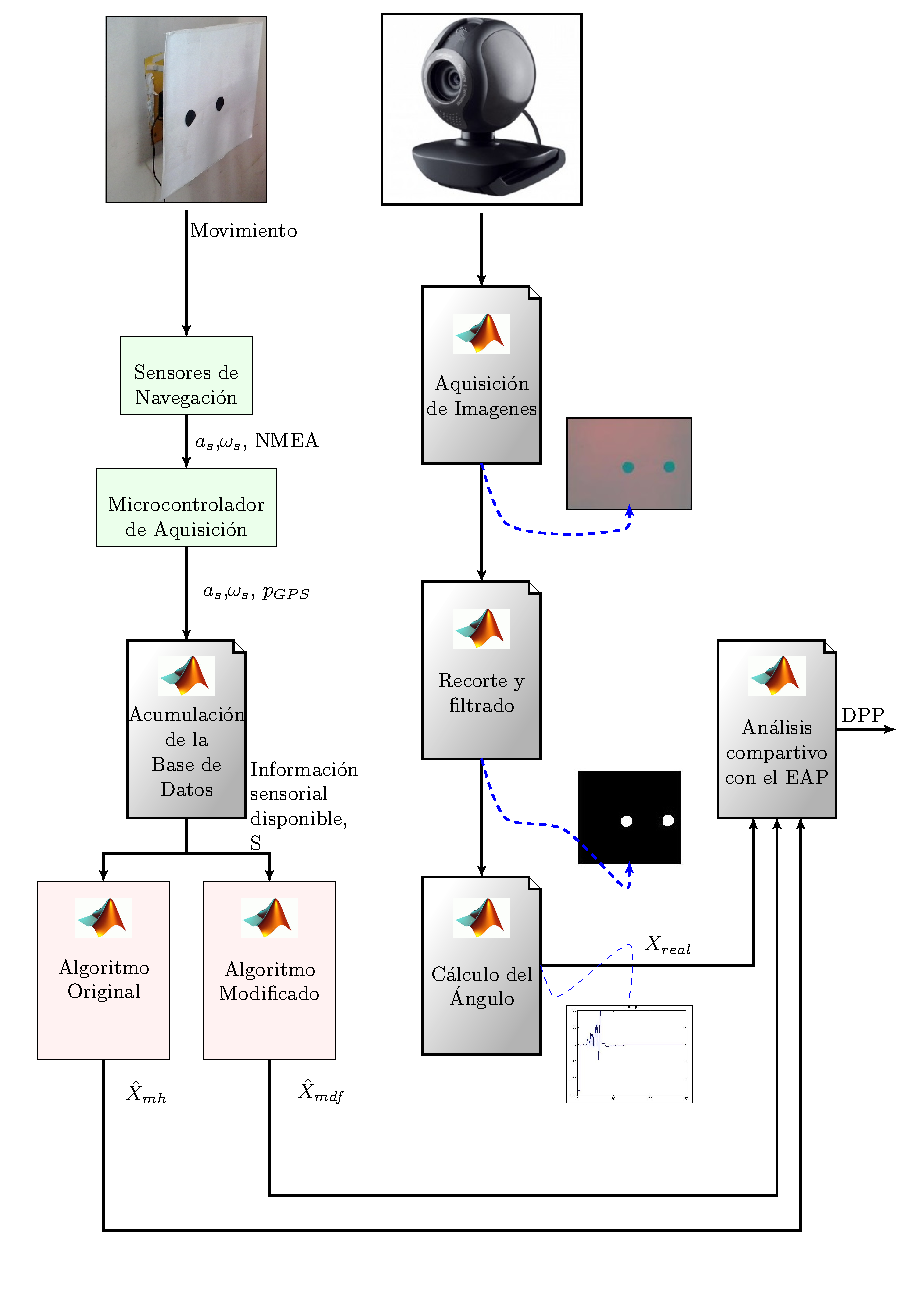
\includegraphics[width=20em]{plataforma_fig10.pdf}
\caption{Esquema general de la plataforma experimental evaluativa.}
\scriptsize{Fuente: Elaboración Propia}
\label{plataforma_fig10}
\end{figure}
La plataforma experimental de la estimación de los ángulos de Euler fue implementada siguiendo el esquema de la Figura \ref{plataforma_fig10}, donde un arreglo de marcas negras en una plancha blanca sujeta a la caja de sensores permite hacer el seguimiento de la evolución del movimiento angular de manera simultánea a la captura de las señales de los sensores de navegación. De esa manera el procesamiento está dividido en dos etapas: primero se sigue el procedimiento descrito en la Figura \ref{plataforma_fig1}, por el cual se obtiene la estimación de la información de navegación $\hat{X}_{mdf}$ y $\hat{X}_{mh}$; posteriormente, de forma paralela se obtiene la información de referencia correspondiente a la evolución temporal de la componente\footnote{De posición angular} sobre la cual se está haciendo el análisis, esta información procede del estudio del desplazamiento de las dos marcas negras capturado en una secuencia de imágenes. La cual es sometida a varios procesos de filtrado para determinar la posición de las marcas y así calcular la progresión de la inclinación equivalente al desplazamiento angular de la variable en estudio, a continuación este procedimiento es descrito en la siguiente secuencia de pasos:
\begin{enumerate}
\item En cada una de las imágenes, para un color en particular\footnote{Se selecciona empíricamente entre las tres matrices de intensidad (rojo, verde y azul) buscando el mejor desempeño en la determinación de las marcas.},  se recorta la zona por donde se mueven las marcas. 
\item Posteriormente, se invierten los colores con la finalidad de resaltar la ausencia de luz\footnote{Debido a su color Negro de las marcas} para después convertirlas en imágenes binarias usando la función \texttt{im2bw(imagen,umbral)} de la \textsl{Image Adquisition Toolbox} de \textsl{MATLAB}, donde el umbral es determinado por prueba-error para cada experimento y condición de iluminación.
\item Con la finalidad de eliminar el ruido introducido por las sombras, en cada una de las imágenes binarias aplicamos el filtro morfológico \texttt{imopen()}, el cual elimina todos los cúmulos aproximadamente circulares con un radio menor a 5 ó 2 pixeles (dependiendo del experimento).
\item Entonces para eliminar totalmente el efecto de las sombras se aplica la función \texttt{imclearborder()}, la cual elimina todas las estructuras morfológicas conectadas al borde.
\item En este punto ya se tiene una secuencia de imagenes depuradas donde solo aparecen las marcas, y corresponde calcular los centriodes de las marcas e identificar cual corresponde a una marca central y cual a una marca externa. Para esto, basados en la función \texttt{colorit()} del apéndice B, se asigna un color a  cada cúmulo\footnote{Que representa a una marca}, despues calculando el centroide se hace la asignación de centro o marca externa basados en cual centroide es más próximo al centro. Este proceso de asignación es seguido en todas las imágenes de la secuencia obteniendo al final dos vectores columna que contienen las coordenadas de las marcas durante todo el desplazamiento.
\item Con los vectores columna de la evolución de la posición vs tiempo tanto del centro como de la marca exterior se determina el ángulo de inclinación, que coincide con la inclinación de los sensores de navegación, ya que la cámara y los sensores están alineados en planos paralelos usando burbujas de albañilería de manera muy cuidadosa.
\end{enumerate}
Esta es una variación del ejemplo \textsl{Length of a Pendulum in Motion} desarrollado por MATLAB. El código implementado en este trabajo se muestra en el apéndice \ref{apen2}.\par
%%
Ahora bien, debido a las características de la plataforma los experimentos desarrollados atacan el análisis de uno de los componentes de los ángulos de Euler a la vez, por lo tanto en cada uno de los ensayos se buscó el cumplimiento de las siguientes condiciones que garantizan que el ángulo determinado en la recta que pasa por los centroides coincida con el ángulo de giro en el parámetro de Euler en cuestión:
\begin{enumerate}
\item El eje de la cámara debe coincidir con el eje de rotación de la caja de los sensores.
\item Dos de los ejes del marco referencial $\marco{A}$ deben formar un plano paralelo al plano de rotación, para así garantizar que el movimiento en los ángulos restantes sea nulo.
\item Y por último, que los ángulos de inclinación de las marcas y la de la caja de sensores estén alineados en cero grados antes de comenzar el movimiento, y así minimizar el bias en la medición del ángulo con la cámara.
\end{enumerate}
Bajo estas condiciones se hacen tres arreglos distintos para los tres ejes del $\marco{B}$, es decir en $x$ para $\phi$, en $y$ para $\theta$, y en $z$ para $\psi$.
\subsection{Plataforma experimental de la estimación de la posición y velocidad lineal}
Para la evaluación de la estimación de la posición y velocidad lineal el esquema implementado utiliza como sensor adicional un GPS Etrex-Garmin que tiene una precisión de hasta 2 metros, por mucho mayor a la del módulo GPS usado dentro del conjunto de sensores de navegación, esto gracias a la ganancia de su antena que le permite capturar un mayor número de satélites, además de tener una memoria especializada para la captura de datos de Efemérides y Calendarios pasados. Este dispositivo cuenta con un altímetro y una brújula electrónica, mejorando su precisión aún más.\par%%
\begin{figure}
\centering
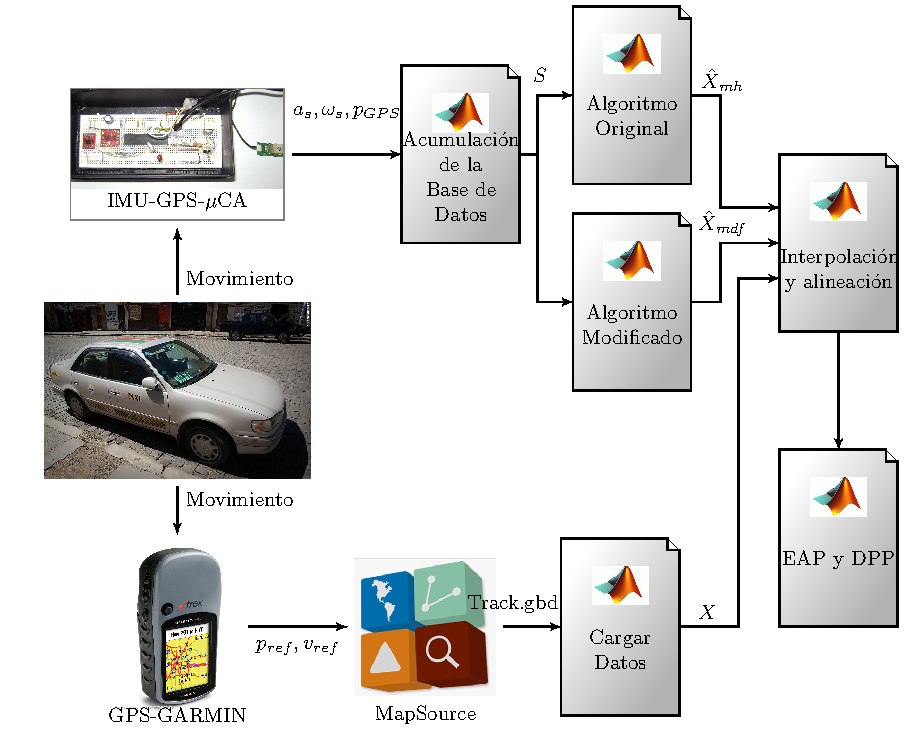
\includegraphics[width=20em]{plataforma_fig11.pdf}
\caption{Plataforma experimental de la estimación del movimiento lineal.}
\scriptsize{Fuente: Elaboración Propia}
\label{plataforma_fig9}
\end{figure}
Los experimentos son realizados siguiendo circuitos cerrados en un vehículo en donde se monta una caja que contiene al sensor adicional y los sensores de navegación de forma tal que es posible realizar la estimación de la información de navegación y capturar información de referencia. El procedimiento seguido para la captura de esta información es mostrado en el esquema de la Figura \ref{plataforma_fig9}, donde el movimiento del vehículo es capturado simultáneamente por el GPS GARMIN-ETEX y los sensores de navegación, incorporando esta información por medio del programa \texttt{adquiereINS.m}, el cual contiene los comandos de comunicación con el microcontrolador de adquisición; posteriormente esta información, debidamente guardada en $S$, es procesada por los algoritmos de navegación sintetizados en los programas \texttt{ProcesamientoMahonyScan.m} y \texttt{ProcesamientoModificado.m}; en lo que corresponde a GPS GARMIN-ETEX, la información de la orientación de la brújula, la magnitud de la velocidad de desplazamiento y la posición en coordenadas geódicas \footnote{Las que son guardadas en la memoria del dispositivo} es guardada en el archivo \texttt{Track.gdb}, luego extraída y reordenada en el archivo \texttt{Track.xls} utilizando el programa \emph{MapSource}, para que finalmente el programa \texttt{CargarDatos.m} extraiga el historial del movimiento lineal en el marco referencial $\marco{A}$; concluyendo con el proceso, los programas \texttt{Sync.m} sincronizan temporalmente la información estimada y la de referencia siguiendo el periodo de muestro $h$, para posteriormente incorporar las fórmulas de cálculo de los EAP y el DPP.
\end{enumerate}
\section{Pruebas experimentales}
Una vez detalladas las plataformas experimentales corresponde hacer la descripción del proceso experimental seguido para indagar en la veracidad de la suposición ya descrita en la Sección \ref{Propuesta} -la cual se constituye en el principal aporte del presente trabajo- la cual afirma que:
\begin{quote}
La inclusión de un Observador Óptimo EKF para la reconstrucción de la matriz de rotación en el esquema de observadores tipo filtro complementario en $SO(3)$ mejora la estimación de la información de navegación.
\end{quote}
La estrategia abordada para cumplir con tal objetivo divide el total de la prueba en dos partes:
\begin{itemize}
\item La prueba para el estudio del desempeño de la estimación de los ángulos de Euler.
\item La prueba para el estudio del desempeño de la estimación de movimiento lineal, es decir la posición y la velocidad lineal.
\end{itemize}
De esa manera, y siguiendo esta secuencia, en esta sección se detalla el procedimiento experimental seguido en la realización de estas dos pruebas.
\subsection{Prueba con la plataforma experimental de la estimación los ángulos de Euler}
Esta fase emplea el esquema experimental descrito en la sección \ref{Plataforma2}, en la cual el sensor angular de video (constituido por una cámara) captura la información de la rotación de uno de los ángulos de Euler, al mismo tiempo que los algoritmos de navegación realizan la estimación de la misma variable\footnote{Dentro del conjunto de datos que conforman la información de navegación estimada.}.\par
%%%
Es importante señalar que debido a que el esquema del sensor angular de video solo puede medir un ángulo al mismo tiempo, el estudio se concreta sobre tres arreglos distintos, en los cuales se varía la disposición de los elementos que constituyen esta plataforma experimental\footnote{Plataforma experimental de la estimación de los ángulos de Euler (ver Figura \ref{plataforma_fig10})}:
\begin{enumerate}
\item \emph{El arreglo para el estudio del ángulo de alabeo $\phi$}. En este los elementos están configurados de tal forma que: el eje de rotación es paralelo al eje $x$ del marco $\marco{B}$; la plancha de las marcas (que se constituye como el plano de rotación) es paralelo al plano $YZ$, con las componentes $z$ apuntando hacia el centro de la tierra y $y$ hacia la izquierda de la imagen\footnote{Cuando la caja de sensores se encuentra con la cara inferior mirando hacia el suelo}. Con lo que respecta a la cámara esta se encuentra en posición vertical tal como se muestra en la Figura \ref{CamAlign}, a una distancia suficiente para enfocar toda la escena de la rotación.
\item \emph{El arreglo para el estudio del ángulo de rodadura $\theta$}. Aquí el eje de rotación es paralelo al eje $y$ del marco $\marco{B}$, el plano de rotación queda en el plano $XZ$, con la componente $z$ (una vez más) apuntando hacia abajo y $x$ apuntando hacia la derecha de la imagen.
\item \emph{El arreglo para el estudio del ángulo de guiñeo $\psi$}. Aquí la configuración cambia radicalmente. En este caso el eje de rotación es paralelo a eje $z$ y perpendicular al plano de rotación sobre el plano $XY$; el versor de $z$ está apuntando hacia abajo en sentido contrario a la posición de la cámara, la cual en este caso está ubicada encima de la caja de sensores; con respecto a los ejes $x$ y $y$, estos apuntan hacia arriba y la izquierda de la imagen tomada por la cámara.
\end{enumerate}
En resumen, en cada uno de los arreglos se realizan varios ensayos, los cuales consisten en la captura de la información de la rotación: en una dimensión para el sensor angular de video, y tres dimensiones para los algoritmos de navegación; de forma tal que tras cada ensayo, si las condiciones de alineación y calibración fueron satisfactoriamente cumplidas, se obtiene como resultado tres señales: la estimación del algoritmo modificado, la estimación del algoritmo original y la medición del sensor angular de video como señal de referencia.\par
El procedimiento seguido en cada uno de los ensayos sigue la siguiente secuencia: primero, se enciende el sensor angular de video; después se mueve la marca externa cerca a los cero grados; se inicia la captura del movimiento junto con el arranque del programa \texttt{AdquiereINS.m}; al terminar la adquisición de los datos, estos se guardan en un archivo \texttt{.mat}; y empleado este archivo, finalmente se procede a calcular las estimaciones de la información de navegación con los programas \texttt{AlgoritmoModificado.m} y \texttt{AlgoritmoOriginal.m}. Aunque entre ensayos varían, en general el movimiento comienza con los ángulos inicialmente alineados\footnote{Esto considerando los dos elementos, es decir la caja de sensores y la plataforma de marcas.} cerca de $0º$, después varían con diferentes velocidades angulares y sentidos de giro durante un periodo de tiempo, el movimiento termina otra vez cerca a los $0º$. En todos los ensayos, se buscó con prioridad mantener los planos de rotación lo más paralelos posible, considerando un ensayo como exitoso solo cuando esta condición se cumple.
%%%
\subsubsection{Resultados de la estimación del ángulo de alabeo.}
Los datos obtenidos de uno de los varios ensayos realizados para esta variable se muestran en la gráfica de la Figura \ref{PlotPh1}, donde la señal de color azul corresponde a la estimación, la de color verde para el  algoritmo original, y de color rojo para la referencia; además, la gráfica superior corresponde a toda la duración del ensayo y la gráfica inferior es el acercamiento del recuadro en color magenta.\par
%%
En este ensayo el movimiento inicia en -2º y termina en poco menos de -3º y los ángulos de rodadura y guiñeo se mantienen en 0º. Para la estimación con el algoritmo modificado los errores oscilan entre $9.04E-4º$ y $10.58º$ en contraste a los $7.33E-3º$ a $18.97º$\footnote{Estos valores están en valor absoluto respecto a la señal original.} para el algoritmo original. 
\begin{figure}
\begin{center}
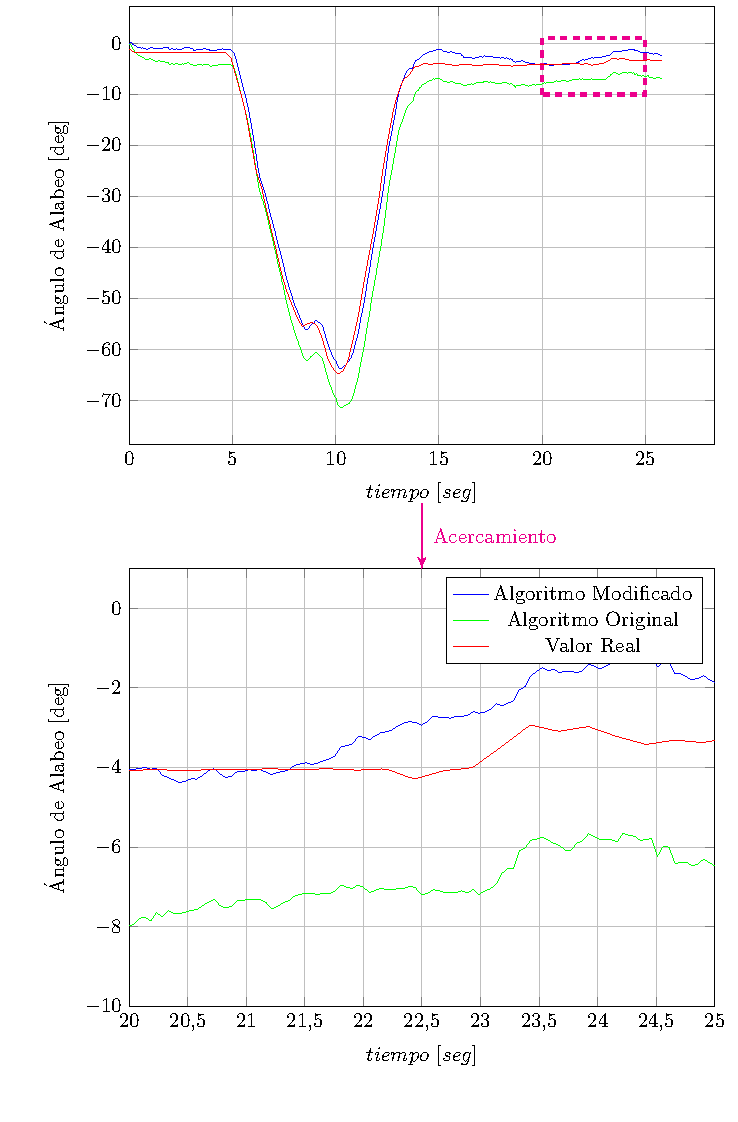
\includegraphics[width=25em]{PlotPh25a.pdf}
\caption{Ángulo de alabeo.}
\label{PlotPh1}
\end{center}
\end{figure}
En promedio los errores absolutos (EAP) para estos algoritmos corresponden:
\begin{equation*}
EAP_{mdf,\phi}=1.3579º~\text{Para el algoritmo modificado.}
\end{equation*}
\begin{equation*}
EAP_{mh,\phi}=3.756º~\text{Para el algoritmo original.}
\end{equation*}
%%%
En estas gráficas los errores cometidos por el algoritmo original son mucho mayores a los del algoritmo modificado, donde este último gana definitivamente a partir de 15 segundos. Es también visible que al final hay una tendencia, para ambos algoritmos de acercarse a la señal de referencia.
\subsubsection{Resultados de la estimación del ángulo de rodadura.}
Los resultados de los ensayos muestran una tendencia de superioridad del método modificado respecto al original. Uno de estos ensayos se muestra en la gráfica de la Figura \ref{PlotPh1}, donde una vez más la gráfica de color azul corresponde a la estimación usando el algoritmo modificado, la de color verde para el algoritmo original y la referencial en color rojo. \par
A diferencia del ensayo mostrado anteriormente, en este ensayo los movimientos son mucho más rápidos, los cuales quedan limitados dentro de la banda de $\pm45[º/s]$. Una vez más en este ensayo, el desempeño del algoritmo modificado mejora sobre al algoritmo original, y a partir de los 13 segundos la convergencia del método modificado es insuperable. En la gráfica de acercamiento (que se delimita por la el rectángulo de color magenta) podemos observar el efecto de un golpe en la caja de sensores que inicia a los 21 segundos, que si bien es accidental muestra el tiempo de convergencia de 4 a 5 segundos para el algoritmo modificado.\par
\begin{figure}
\begin{center}
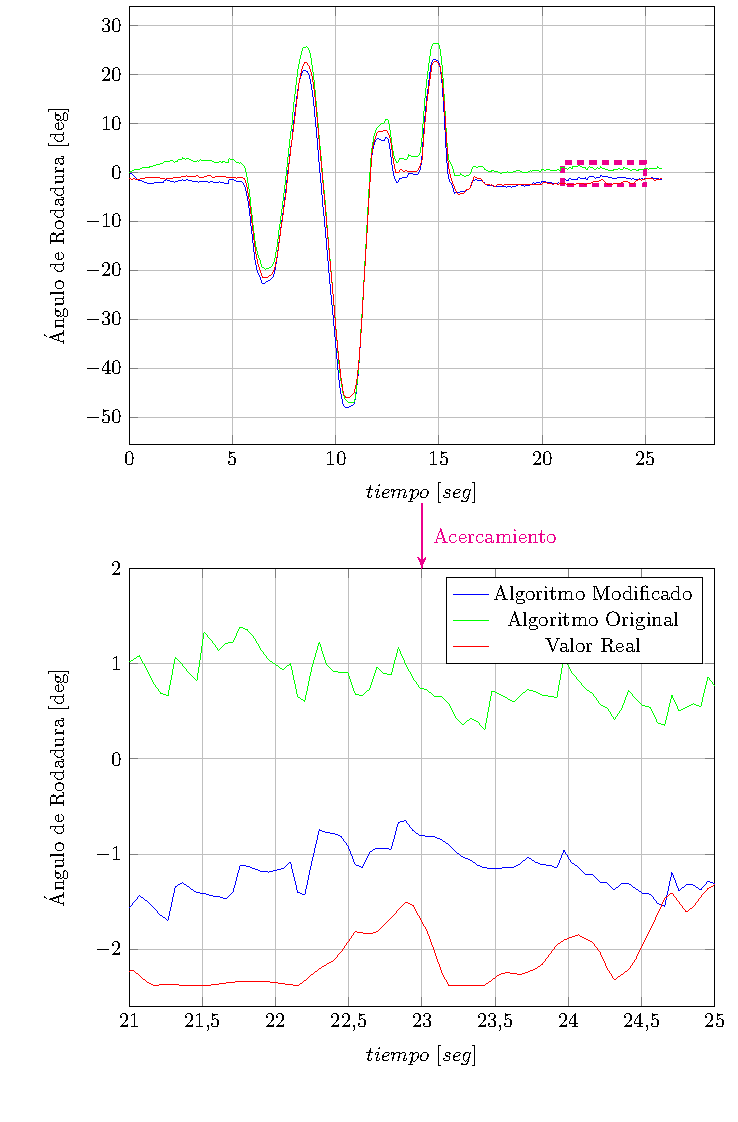
\includegraphics[width=25em]
{PlotTh27.pdf}
\caption{Ángulo de rodadura.}
\label{PlotTh1}
\end{center}
\end{figure}
Ahora los EAP's para este ensayo son:
\begin{equation*}
EAP_{mdf,\theta}=1.4635º~\text{Para el algoritmo modificado.}
\end{equation*}
\begin{equation*}
EAP_{ms,\theta}=7.072º~\text{Para el algoritmo original.}
\end{equation*}
%%%
Una vez más la gráficas muestran que los errores cometidos por el algoritmo original son mucho mayores a los del algoritmo modificado.\par
La convergencia para el método modificado empieza a ser fiel iniciando los 13 a 14 segundos (ver gráfica), en contraste con el método original en el cual la convergencia no llega en la ventana temporal que dura el experimento; aunque parece que al final hay una cierta tendencia. \par
%%
Ahora, es posible que esto de deba a que a pesar de haber reducido el error constante en la medición durante el proceso de calibración del arreglo, queden residuos que favorezcan al método modificado; si este es el caso, se ve que el golpe no perturba en demasía el valor final encontrado por el algoritmo original, de lo cual podemos decir que tiene cierto grado de robustez superior a la desempeñada por el algoritmo modificado.\par 
%%%
\subsubsection{Resultados de la estimación del ángulo de guiñada}
Para la componente de guiñada los ensayos fueron realizados con la plataforma en posición horizontal dando al sistema mayor movilidad. Con estas características, en este arreglo se pudieron alcanzar velocidades angulares mucho mayores a la de los otros experimentos. Sin embargo, se hace importante mencionar que en estas condiciones el vector gravitacional está apuntando paralelo al eje de rotación, dificultando la estimación vectorial y así la estimación del ángulo de guiñeo para el algoritmo original; por esta razón la capacidad de convergencia del método original, cuando la condición inicial del ángulo muy distinta de cero, se ve afectada considerablemente.\par
%%
En la Figura \ref{PlotPs1} se muestra los resultados de la estimación del ángulo de guiñeo. Específicamente en este experimento el ángulo inicial de guiñeo es de 5º, lo que permite ver el efecto anteriormente mencionado, donde a pesar de que las condiciones iniciales de los ángulos de Euler en los algoritmos de navegación son nulas, el algoritmo modificado reduce progresivamente el error, en contraste con el algoritmo original, el cual permanece con un error constante de 1.5º (como se muestra en el acercamiento), por lo menos durante toda la ventana temporal que dura el experimento.\par
\begin{figure}
\begin{center}
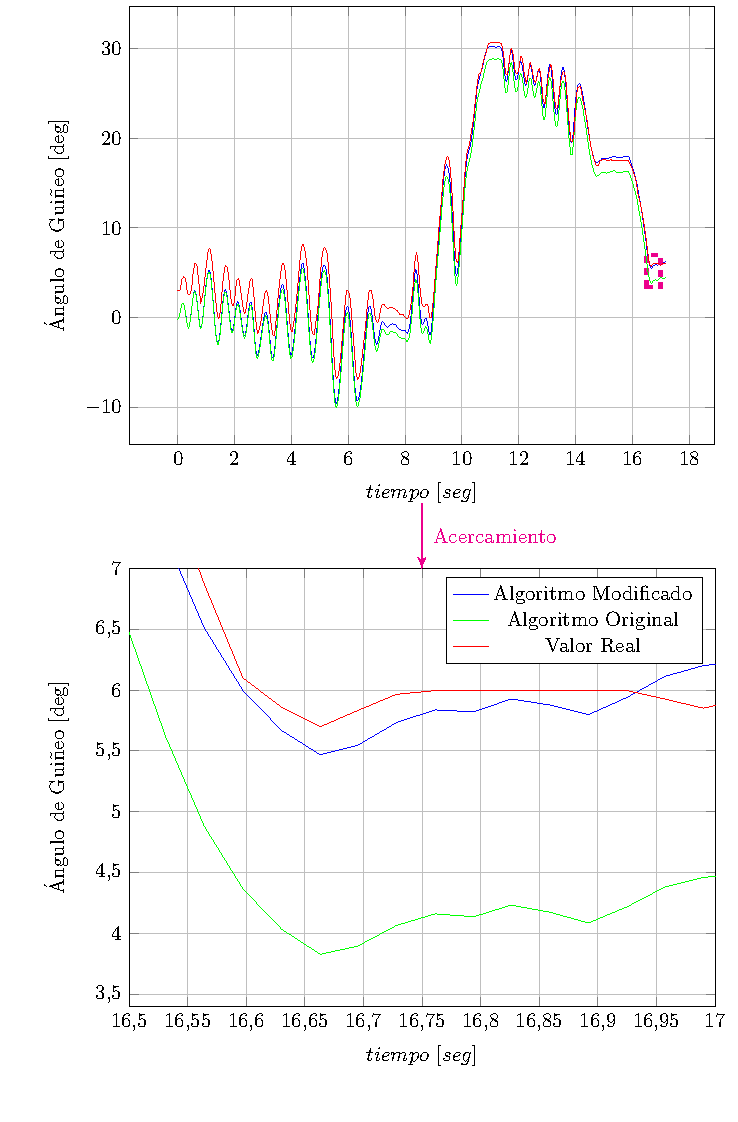
\includegraphics[width=25em]{PlotPs11.pdf}
\caption{Ángulo de guiñeo.}
\label{PlotPs1}
\end{center}
\end{figure}
En cuanto al tiempo de convergencia, de forma reiterada en todos los ángulos muestra que la convergencia siempre está cerca de los 12 segundos, y a partir de ese tiempo se sigue fielmente la referencia.\par
En este ensayo los EAP simplemente corroboran la evidente ventaja de método modificado frente al original.
\begin{equation*}
EAP_{mdf,\psi}=1.4635º~\text{Para el algoritmo modificado.}
\end{equation*}
\begin{equation*}
EAP_{ms,\psi}=7.072º~\text{Para el algoritmo original.}
\end{equation*}\newpage
\subsection{Prueba con la plataforma experimental de la estimación del movimiento lineal}
Los experimentos realizados con esta plataforma permiten ver el desempeño del algoritmo para estimar el movimiento lineal, es decir la velocidad lineal y la posición en el tiempo. \par
\begin{figure}[ht]
\begin{center}
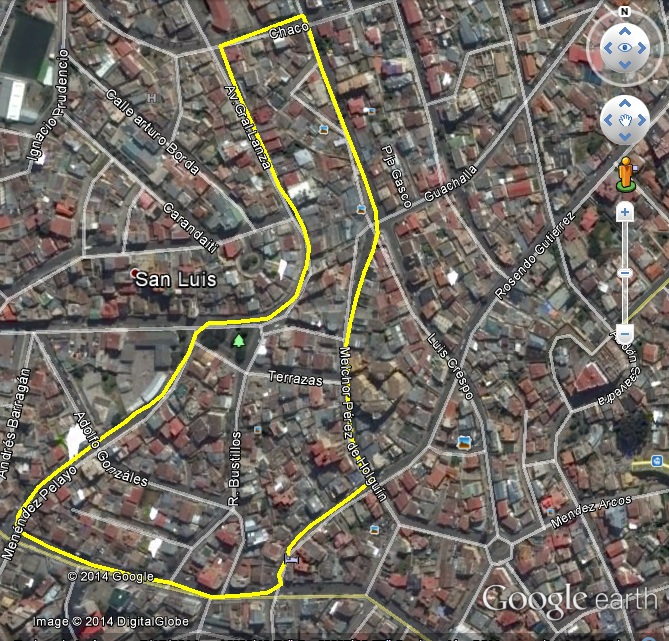
\includegraphics[width=25em]
{pruebas_fig1a.jpg}
\caption{Circuito cerrado \scriptsize{Fuente: Google Earth y DigitalGlobe 2013}}
\label{pruebas_fig1}
\end{center}
\end{figure}
Los ensayos se desarrollan en un circuito cerrado delimitado en la zona de Sopocachi Alto\footnote{Zona seleccionada por sus facilidades logísticas.} con los sensores montados en un vehículo. Esta ruta, mostrada en la Figura \ref{pruebas_fig1}, tiene una longitud de $1.53[Km]$, pasa por calles con buena línea de vista, sin muchos árboles\footnote{Podados por la época del año.} ni edificios. En cada ensayo se siguió el siguiente protocolo:	
\begin{enumerate}
\item Se hace la alineación al norte tanto del GPS-GARMIN-ETREX, como la del marco referencial $\marco{B}$, para que las condiciones iniciales en los ángulos de Euler sean nulas.
\item Se inicia el programa de \texttt{AdquiereINS.m}.
\item Se hace el desplazamiento con velocidades de hasta $20[kph]$.
\item Y por último se guarda los datos adquiridos para comenzar con el siguiente ensayo, si corresponde.
\end{enumerate}
A continuación se describen los resultados obtenidos de las pruebas que se pudieron realizar, señalando que no fueron muchas debido a un tema de disponibilidad de equipos.
\subsubsection{Resultados de la estimación de la posición}
Como ya se señala las pruebas fueron realizadas en un radiotaxi siguiendo la ruta de la Figura \ref{pruebas_fig1}. En esta ruta las calles con mayor conflicto de línea de visión del GPS debido a la proximidad de los edificios fueron la c/ Melchor Pérez de Holguín y la c/ Chaco.\par
%%
\begin{figure}
\begin{center}
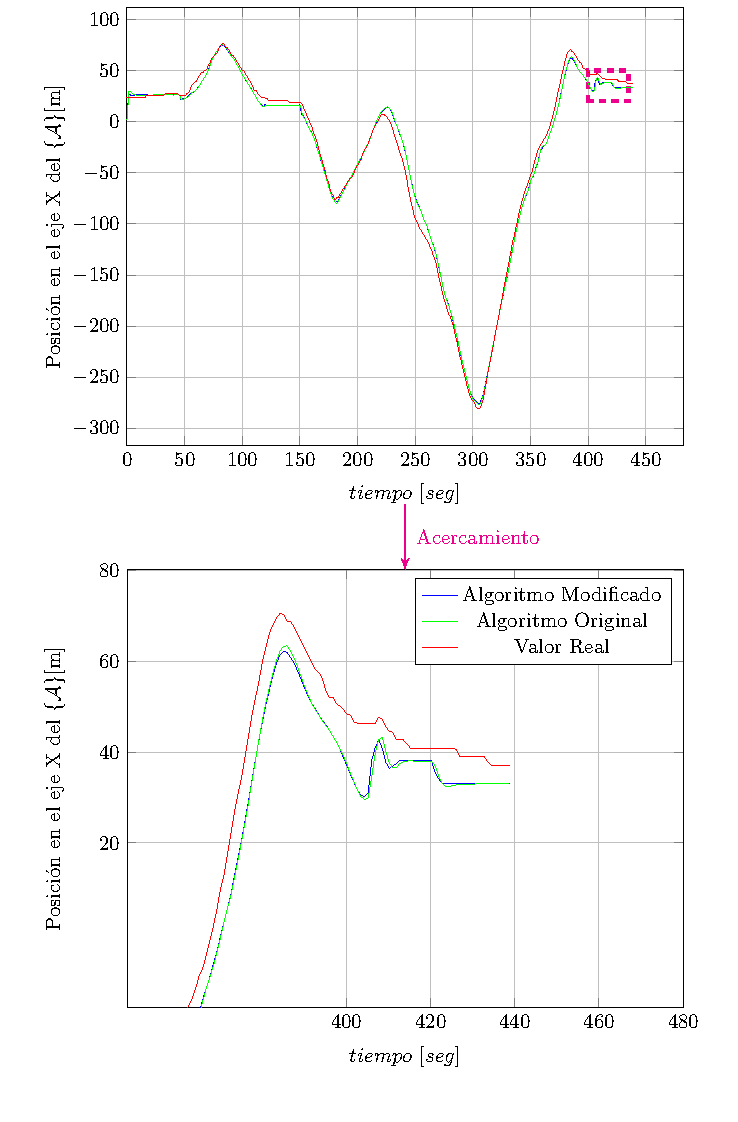
\includegraphics[width=25em]
{PlotX4b.pdf}
\caption{Posición en el eje X.}
\scriptsize{Resultados de la estimación de con datos simulados. Resultados típicos del repetidos intentos.}
\label{PlotX1}
\end{center}
\end{figure}
%%
\begin{figure}
\begin{center}
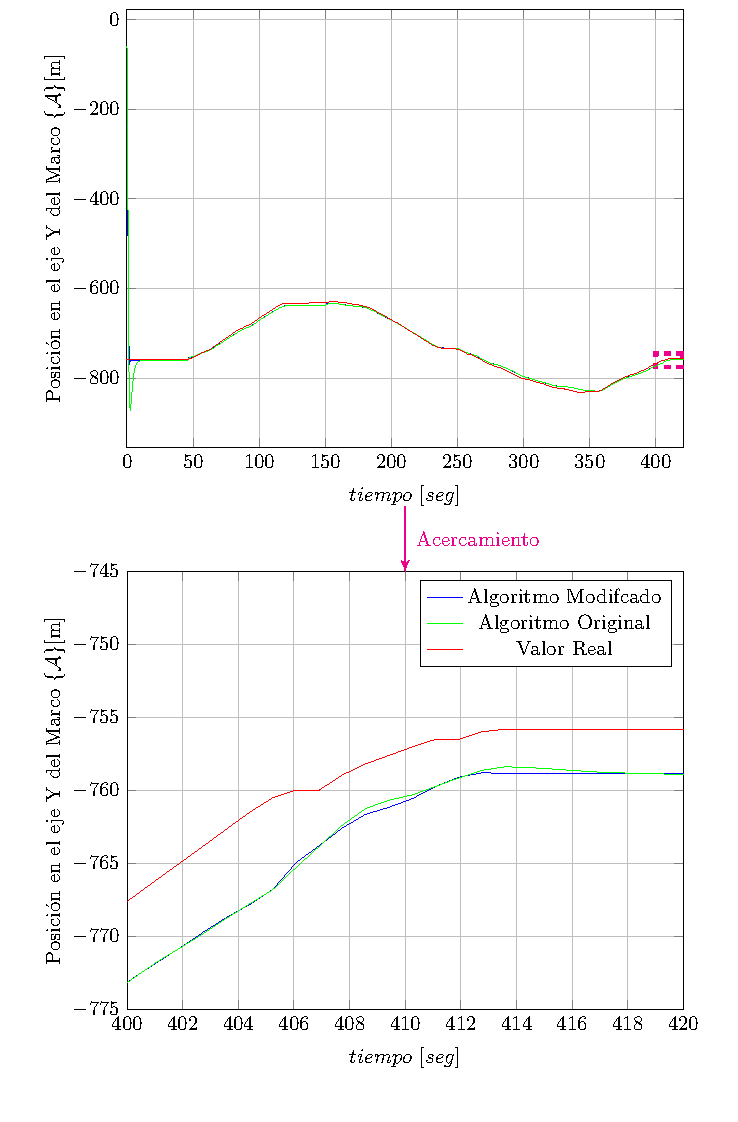
\includegraphics[width=25em]
{PlotY4b.pdf}
\caption{Posición en el eje Y.}
\scriptsize{Resultados de la estimación de con datos simulados. Resultados típicos del repetidos intentos.}
\label{PlotY1}
\end{center}
\end{figure}
%%%
\begin{figure}
\begin{center}
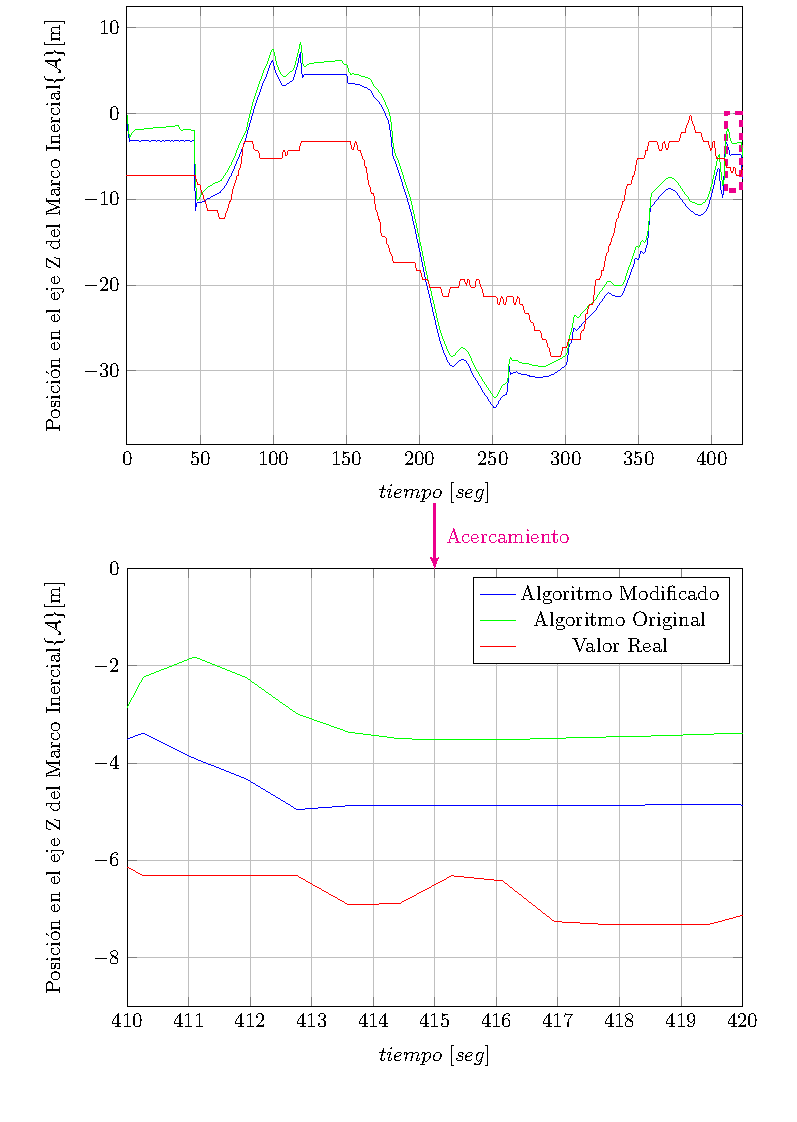
\includegraphics[width=25em]
{PlotZ4b.pdf}
\caption{Posición en el eje Z.}
\scriptsize{Resultados de la estimación de con datos simulados. Resultados típicos del repetidos intentos.}
\label{PlotZ1}
\end{center}
\end{figure}
%%%
En todas las gráficas, los resultados de la estimación del algoritmo Original son representados en la línea de color verde, para la estimación del algoritmo modificado de color azul, y para la señal de referencia en una línea de color rojo. Estos resultados son mostrados en las Figuras \ref{PlotX1}, \ref{PlotY1} y \ref{PlotZ1}. Este ensayo dura 421 segundos ó 7 minutos 1 segundo, y durante todo este tiempo se puede observar, que si bien la estimación sigue la señal de referencia esta mantiene un error durante toda la trayectoria, esto para ambos algoritmos. Sin embargo, dado que la diferencia entre las dos estimaciones es muy pequeña, el tema del error no afecta a la suposición que se trata de refutar o afirmar, dado que se habla de cual de los algoritmos estima mejor, y a pesar de que ambos estén equivocados, la competencia está en cual es más próximo al valor verdadero.\par
%%
Por su parte, este error puede ser cuantificado en el EAP para cada una de las gráficas, donde el sub-índice $mdf$ significa que pertenece al algoritmo modificado y $mh$ significa que pertenece al algoritmo original:
\begin{equation*}
EAP_{mdf,x}=5.8290 [m]~\text{Para el algoritmo modificado.}
\end{equation*}
\begin{equation*}
EAP_{ms,x}=5.8976 [m]~\text{Para el algoritmo original.}
\end{equation*}
\begin{equation*}
EAP_{mdf,y}=3.5046 [m]~\text{Para el algoritmo modificado.}
\end{equation*}
\begin{equation*}
EAP_{ms,y}=4.6888 [m]~\text{Para el algoritmo original.}
\end{equation*}
\begin{equation*}
EAP_{mdf,z}=6.1602 [m]~\text{Para el algoritmo modificado.}
\end{equation*}
\begin{equation*}
EAP_{ms,z}=6.2365 [m]~\text{Para el algoritmo original.}
\end{equation*}
Respecto a las gráficas de las Figuras \ref{PlotX1} y \ref{PlotY1}, la gráfica de la Figura \ref{PlotZ1} parece la más imprecisa, sin embargo hay que considerar que los errores en la altitud son uno de los mayores defectos del sistema GPS, y típicamente son grandes\footnote{Esto no pone en cuestión la veracidad de la información entregada por el GPS-Garmin, debido a que este dispositivo utiliza la información de un barómetro, que sin duda tiene mejor precisión.}. A pesar de eso, es de consideración ver que la información estimada se aproxima a la señal de referencia, mucho más que la medición del sensor de navegación GPS-MTK3329. 
\subsubsection{Resultados de la estimación de la velocidad lineal.}
En esta prueba, dado que la velocidad de referencia esta expresada en el marco referencial inercial $\marco{A}$ y la medición de la aceleración, de donde se obtiene la estimación, está expresada en el marco referencial fijo al cuerpo $\marco{B}$, se hace inevitable utilizar la matriz de rotación $R$ (definida en la sección \ref{RotationMatrix}) para hacer la transformación correspondiente. Entonces, esto sugiere que la convergencia está delimitada por la capacidad de los algoritmos para estimar los ángulos de Euler. Los resultados de las pruebas realizadas son mostrados en las Figuras \ref{PlotU1}, \ref{PlotV1} y \ref{PlotW1}, en las que se muestran la velocidad en $x$, $y$ y $z$ del marco referencial inercial $\marco{A}$ con la misma notación de colores que se ha venido manteniendo desde la Figura \ref{PlotPh1}.\par
\begin{figure}
\begin{center}
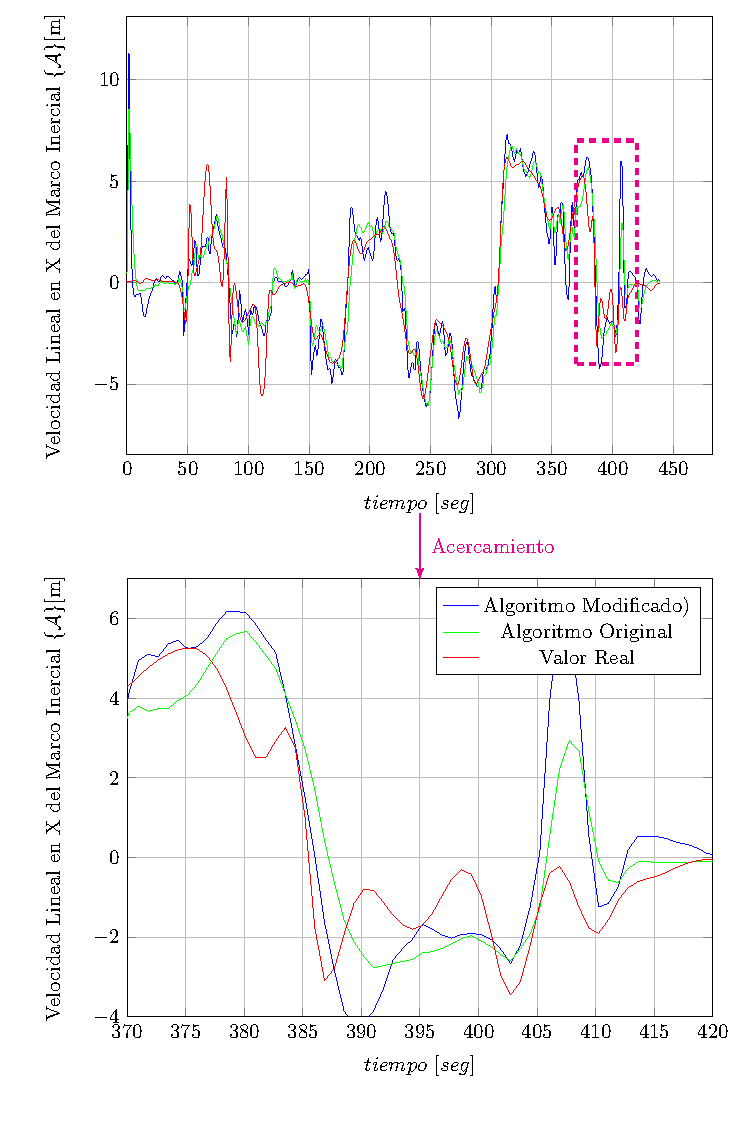
\includegraphics[width=25em]
{PlotU.pdf}
\caption{Velocidad lineal en el eje X.}
\scriptsize{Resultados de la estimación de con datos simulados. Resultados típicos del repetidos intentos.}
\label{PlotU1}
\end{center}
\end{figure}
%%%
En estas gráficas, a pesar de que los errores de la estimación de la posición son bastante grandes\footnote{Para ciertas aplicaciones.}, la estimación de la velocidad parece mucho más certera. Y se observa una ventaja evidente del método modificado frente al original, lo que es positivo para la suposición investigada. Este argumento se refuerza con los valores de los errores absolutos promedio para cada una de las tres variables, denotados a continuación:
\begin{equation*}
EAP_{mdf,u}=0.8958 [m/s]~\text{Para el algoritmo modificado.}
\end{equation*}
\begin{equation*}
EAP_{ms,u}=0.7871 [m/s]~\text{Para el algoritmo original.}
\end{equation*}
\begin{equation*}
EAP_{mdf,v}=3.1564 [m/s]~\text{Para el algoritmo modificado.}
\end{equation*}
\begin{equation*}
EAP_{ms,v}=3.3291 [m/s]~\text{Para el algoritmo original.}
\end{equation*}
\begin{equation*}
EAP_{mdf,w}=0.3476 [m/s]~\text{Para el algoritmo modificado.}
\end{equation*}
\begin{equation*}
EAP_{ms,w}=0.64 [m/s]~\text{Para el algoritmo original.}
\end{equation*}
\begin{figure}
\begin{center}
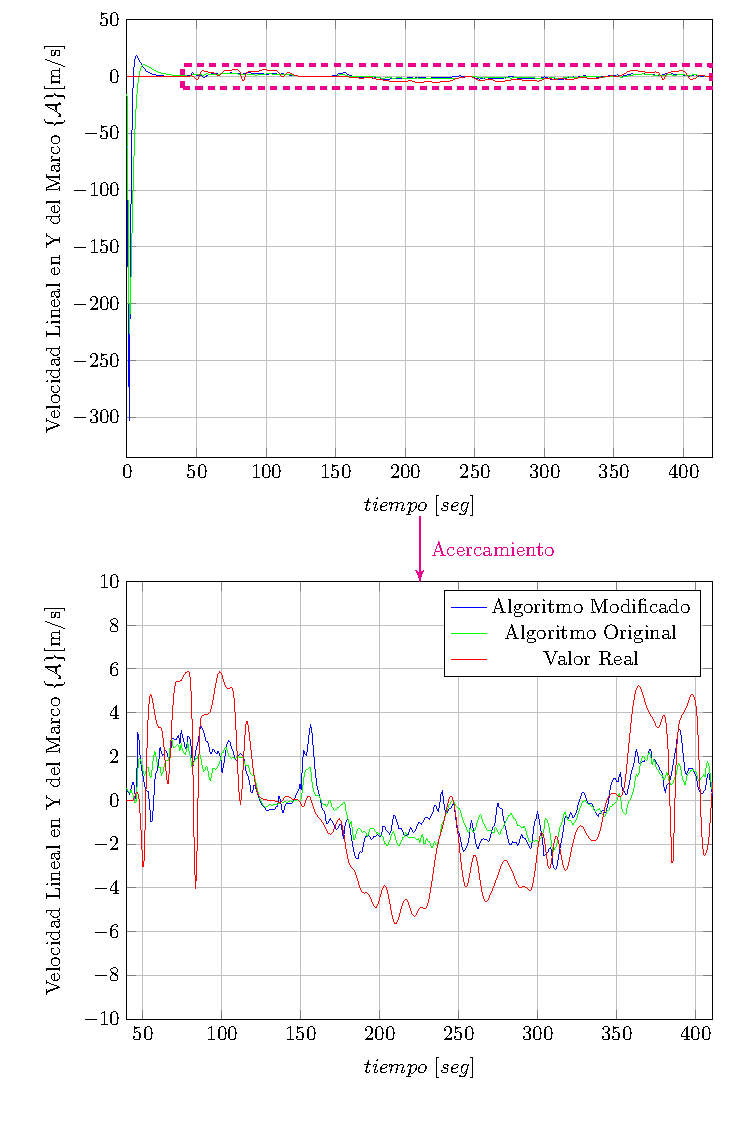
\includegraphics[width=25em]
{PlotV.pdf}
\caption{Velocidad lineal en el eje Y.}
\scriptsize{Resultados de la estimación de con datos simulados. Resultados típicos del repetidos intentos.}
\label{PlotV1}
\end{center}
\end{figure}
%%%
\begin{figure}
\begin{center}
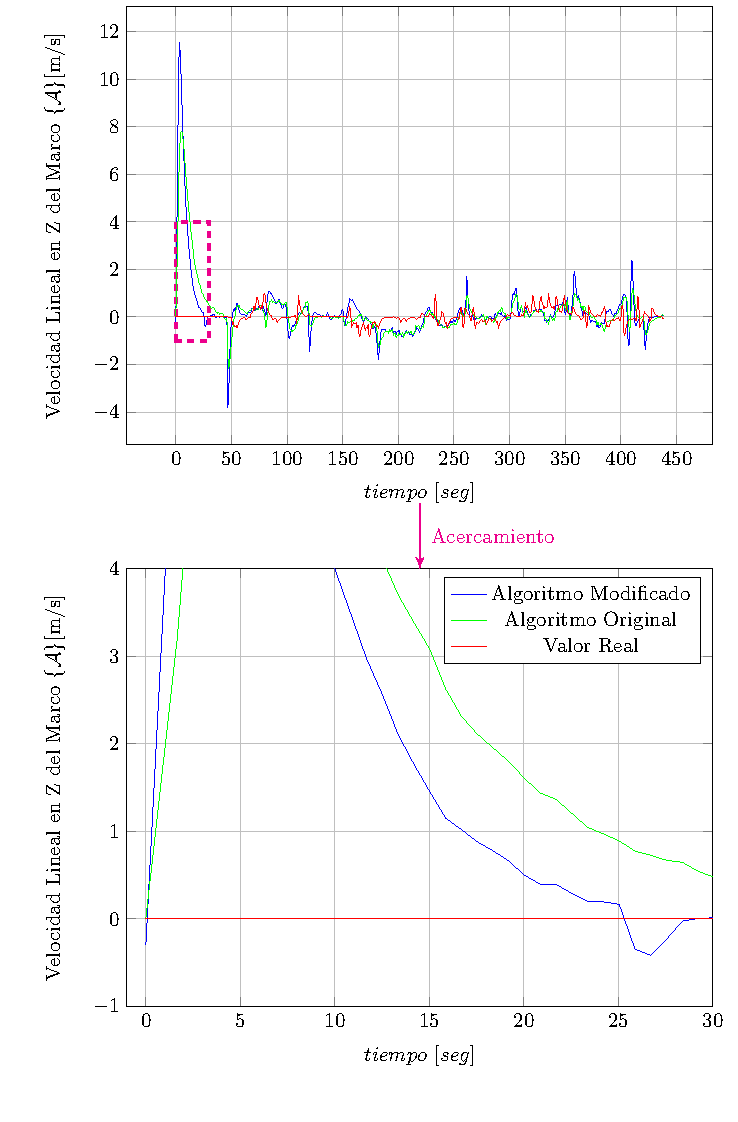
\includegraphics[width=25em]
{PlotW.pdf}
\caption{Velocidad lineal en el eje Z.}
\scriptsize{Resultados de la estimación de con datos simulados. Resultados típicos del repetidos intentos.}
\label{PlotW1}
\end{center}
\end{figure}
\newpage
\subsection{Resultados del Análisis Comparativo con el EAP y el DPP.}
Como se menciona en la anterior sección después de obtener las señales estimadas por los algoritmos de navegación se prosigue con el análisis comparativo con el EAP y el DPP. En la Tabla \ref{resultados_tb1} se ordenan los EAP y las diferencias porcentuales para cada variable.\par
\begin{table}
\begin{center}
\begin{tabular}{|p{2in}|p{1.0in}|p{1.0in}|p{1.0in}|} \hline
\textbf{Variable estimada}&\small\textbf{Error Absoluto Promedio del algoritmo modificado}&\small\textbf{Error Absoluto Promedio del algoritmo original}&\small\textbf{Diferencia Porcentual del Algoritmo Modificado respecto al Original.} \\ \hline
%--------------------------------------------------------------------->
Posición en el eje X ($x$) &5.8862[m]&5.9427[m]&0.9596\%\\ \hline
Posición en el eje Y ($y$) &3.5445[m]&4.7739[m]&34.6828\%\\ \hline
Posición en el eje Z ($z$)&6.1698[m]&6.3369[m]&2.7080\%\\ \hline
Velocidad lineal en el eje X ($v_x$) &0.8214[m/s]&0.7871[m/s]&{-12.1305\%}\\ \hline
Velocidad lineal en el eje Y ($v_y)$&3.1564[m/s]&3.3291[m/s]&5.4710\%\\ \hline
Velocidad lineal en el eje Z ($v_z$)&0.4445[m/s]&0.5697[m/s]&28.1664\%\\ \hline
Ángulo de alabeo ($\phi$ )&1.3579[Deg]&3.7560[Deg]&177.97\%\\ \hline
Ángulo de rodadura ($\theta$ )&1.4635[Deg]&2.801[Deg]&91.394\%\\ \hline
Ángulo de guiñeo ($\psi$ )&1.3268[Deg]&2.1855[Deg]&44.53\%\\ \hline
\end{tabular}
\caption{Tabla comparativa del desempeño de Algoritmo de tres observadores en cascada y el de Mahony-Scandaroli.}
\label{resultados_tb1}
\end{center}
\end{table}
En esta tabla se puede ver globalmente que el algoritmo modificado es superior en casi todas las variables, lo que se corrobora con el cálculo del DPP que se denota como:
\begin{equation}
DPP=40.92\%
\end{equation}
Fríamente, el DPP indica que en promedio se tiene 40.92\% mejor desempeño en la estimación de la información de navegación para el algoritmo modificado respecto al original.\par
%%
Analizando los pares de EAP mostrados en la Tabla \ref{resultados_tb1} vemos una marcada tendencia que indica que el algoritmo modificado supera al algoritmo original. Dentro de las diferencias más relevantes se tienen: la estimación de la posición en el eje $y$  con $1.22[m]$ de distancia en promedio, y los ángulos de alabeo y rodadura, con $2.39º$ y $1.73º$, respectivamente.\par
%%
En el par de la estimación de la velocidad del eje $X$, marcada de color rojo se muestra un resultado negativo, que indicaría que (para este parámetro) el algoritmo original tiene una ventaja del $12.1305\%$ mejor que el algoritmo modificado. Aunque realmente esto significa que algoritmo modificado fallo en $0.1727[m/s]$ en promedio más que el algoritmo original, lo cual no es muy relevante.\par
\subsection{Tiempos de Procesamiento.}
%%
En relación a los tiempos de procesamiento, se utiliza la función \texttt{tic-tac} de \textsl{MATLAB} para medir el tiempo que le toma a la computadora realizar el procesamiento de todo el conjunto de muestras.\par
%%
Sin embargo, se debe tener cuidado con la información que esta función pueda dar. Esto debido a que la memoria virtual asignada al proceso \textsl{MATLAB} es limitada y su acceso es compartido con los otros procesos del sistema; además, el direccionamiento de la misma -a medida que se llena- requiere un mayor número de accesos. Por esta razón, el tiempo de procesamiento, por ejemplo, de 1.000 datos no guarda una relación lineal con respecto a 30.000 datos, y los tiempos en cada bucle se incrementan en proporción al número de accesos a la memoria virtual. Sin embargo, para pequeñas cantidades de datos, el tiempo de procesamiento en cada bucle es aproximadamente el mismo. Dicho esto solo se consideran los tiempos de procesamiento para pequeñas cantidades de datos.\par
%%
Estas en promedio para $49.4311 [s]$ es decir $2,957$ puntos de muestreo, el procesamiento demora en promedio: $1.0158[s]$ para el algoritmo modificado y $0.7954 [s]$ para el algoritmo original, definiendo una diferencia porcentual promedio de:
\begin{equation}
DPP_{\texttt{tiempo de procesamiento}}=-21.6933\%
\end{equation}
Lo que indica que el algoritmo original utiliza $21.6933\%$ menos tiempo que el algoritmo modificado.
\section{Análisis y discusión de los resultados.}
El estudio realizado en el presente trabajo permite obtener las gráficas comparativas en las que se despliegan los datos de la estimación junto con los referenciales; se obtienen las tablas de los EAP y DPP relacionados con los errores cometidos por ambos algoritmos; y además los tiempos de procesamiento promedio para los dos algoritmos de navegación. Asimismo, nos permite verificar la validez de varios conceptos introducidos, como el Bloque de Combinación, la discretización de los algoritmos de navegación, el diseño de las matrices de peso en el Observador Óptimo EKF, etc. En este capítulo se aborda más detalladamente los resultados del trabajo.\par
\section{Resultados de diseño.}
La arquitectura propuesta tiene muchas semejanzas con el enfoque del sistema de navegación propuesto por \cite{Kong2004}; pero en las condiciones propuestas en dicho trabajo, la determinación de las variables de navegación corregidas depende del tiempo de disponibilidad de la medición de la posición (con GPS). Esto, al contrario del enfoque propuesto en el presente trabajo, en el cual la corrección es continua y no depende de la disponibilidad de los datos del GPS.\par
%%
Basados en las características de la estimación de la posición, se puede decir que el algoritmo modificado mejora la determinación de la posición sobre el GPS (principalmente en la determinación de la altura, ver Figura \ref{PlotW1}). Sin embargo, si este desempeño es comparado, por ejemplo, con \cite{Cai2011}, en donde el error promedio en la determinación del movimiento lineal es de $2.5 [m]$ y $0.5 [m/s]$\footnote{Para la posición y la velocidad, respectivamente.}, se puede decir que el desempeño del enfoque propuesto es mucho menor. A pesar de esto, se puede ver que existe una mejora en la determinación de la orientación para el algoritmo propuesto, si comparamos los errores promedio en la determinación de los ángulos de Euler (de $1.38[Deg]$ para el presente enfoque, frente a los $1.5[Deg]$ del enfoque de \cite{Cai2011}). No obstante, estas relaciones necesitarían ser probadas en las mismas condiciones y con la misma información de entrada, y por esa razón no se puede decir que los errores reportados en \cite{Cai2011} son comparables con los del presente trabajo .\par
%%
El enfoque abordado para la determinación de las matrices de peso en el algoritmo del Observador Óptimo EKF parece infructuoso, ya que para encontrar una sintonización adecuada estos valores tuvieron que ser reducidos drásticamente. Asimismo, la capacidad de encontrar estos valores depende de la resolución en el dominio de las ponderaciones. A pesar de esto, al incorporar los valores determinados desde el enfoque propuesto en la Sección 3.3, el algoritmo modificado es capaz de llegar a la referencia, pero muy por debajo del desempeño del algoritmo original. Todos estos factores parecen apuntar a que el método de sintonización de las matrices de peso debería considerar primero el mejor desempeño de la estimación para el Observador Óptimo\footnote{En función a costo de los errores cometidos para un conjunto de datos de entrenamiento}; y en una segunda etapa ajustar el desempeño del Observador tipo Filtro complementario en $SO(3)$. \par
%%
El enfoque de discretización de los algoritmos original y modificado, de acuerdo al desempeño alcanzado respecto a la implementación en \cite{Mahony2008}, ha demostrado ser bastante precisa a pesar de que los resultados de ambos enfoques no son comparables\footnote{Esto bajo el argumento de que, al diferir sus señales de entrada, ambos algoritmos no estas sometidos a las mismas condiciones.}.
De todas maneras, el desempeño positivo de la discretización es innegable, y demuestra que la incorporación de términos de la serie de Taylor superiores al grado tres no promete grandes mejoras.\par
%%%%%%%%%%%%%%%%%%%%%%%
\section{Resultados de la experimentación.} %%
%%%%%%%%%%%%%%%%%%%%%%%
La convergencia para la estimación de la orientación del método propuesto en el presente trabajo se verifica con el análisis visual de las gráficas de las Figuras \ref{PlotPh1}, \ref{PlotTh1} y \ref{PlotPs1}. En general, las aproximaciones son bastante cercanas y alcanzan la referencia definitivamente a partir de los doce segundos reduciendo el error. Esto marca una indicación positiva para la inclusión del observador óptimo en la estructura de los filtros complementarios en $SO(3)$.\par
%%
Respecto a la estimación del movimiento lineal, los resultados no son del todo alentadores. En algunos casos el error puede llegar hasta $20[m]$, con un promedio de $5.2[m]$ y en los mejores casos se mantiene dentro de los dos metros de error. Esto reduce en gran medida el rango de aplicaciones del algoritmo, así como está planteado. Y deja la imperante necesidad de incorporar un segundo método de estimación en la determinación de la posición, por ejemplo, como el reportado en \cite{Merwe2004}. A pesar de este comportamiento, la estimación de la velocidad permite pensar en aplicaciones de control en aeronaves no tripuladas (Unmanned Aircraft Vehicles, UAVs), ya que los errores no son demasiado desproporcionados. Además, refiriéndonos a los errores de la posición en los ejes X y Y de la Figura \ref{resultados_tb1}, se acerca mucho al error típico del GPS usado \cite{Mediatek2009} cuyo valor es de 5m en 2D comparado al 4.71 [m], y seguramente en mejores condiciones de visibilidad\footnote{Que típicamente se encuentran en las zonas abiertas en las que los UAV aplicados a vigilancia o exploración funcionan.} el algoritmo promediaría mejores condiciones de estimación.\par
%% 
Existen limitaciones respecto a las entradas, y cuando estas se saturan afectan en gran manera los resultados del observador, por lo tanto el INS solo funciona bajo condiciones en que los vehículos y personas promedio están sometidas; por ejemplo una carretera interdepartamental, un viaje aéreo comercial.\par
%%
Ahora surge la pregunta de si nuestro algoritmo es más o menos complejo que el original, y que: si bien incrementa la calidad de estimación, también incrementa el tiempo de procesamiento? En tal caso la respuesta es aseverativa, y sí, nuestro algoritmo incrementa la complejidad y por ende el tiempo de procesamiento del mismo. Esto se demuestra usando la función \emph{tic-tac} de \textsl{MATLAB}, en las que para las señales mostradas en el capítulo anterior, se tiene un tiempo de procesamiento promedio de $24.6714[s]$ para nuestro algoritmo y 20.274[s] para el algoritmo original. A simple vista este +21.6933\% de tiempo de procesamiento parecería aminorar el progreso logrado por el algoritmo propuesto, pero si por ejemplo el algoritmo original tuviese que ejecutar en tiempo real 1,000,000 de instrucciones en ensamblador para una sola iteración, entonces nuestro algoritmo tuviese 1,200,000 instrucciones, ahora si se considera, por ejemplo el microcontrolador \texttt{PIC24HJ32GP202-I/SP} de 16bits @ 40MIPS, las frecuencias de muestreo corresponden a 60[Hz] y 30.79[Hz], respectivamente; esto significa constantes de tiempo que el algoritmo modificado puede manejar son de hasta 0.0053[s], que cómodamente entran por ejemplo: para la medición de la frenada de un automóvil que es de que tienen constantes de tiempo de hasta 0,18[s], y fácilmente permite proponer el uso en una gran cantidad de vehículos; entonces según este último análisis realmente si se cuenta con una buena capacidad de procesamiento, no es prohibitiva la complejidad introducida por el algoritmo modificado.\par
%%
Según estos datos, el algoritmo modificado es capaz de computar las trayectorias con tan buena precisión como tenga nuestro sensor de posición. Sin embargo el tema de alineación inicial es vital para tener una buena estimación, a pesar de que esto no afecta la estabilidad del sistema en ninguna escala.
% An example of a floating figure using the graphicx package.
% Note that \label must occur AFTER (or within) \caption.
% For figures, \caption should occur after the \includegraphics.
% Note that IEEEtran v1.7 and later has special internal code that
% is designed to preserve the operation of \label within \caption
% even when the captionsoff option is in effect. However, because
% of issues like this, it may be the safest practice to put all your
% \label just after \caption rather than within \caption{}.
%
% Reminder: the "draftcls" or "draftclsnofoot", not "draft", class
% option should be used if it is desired that the figures are to be
% displayed while in draft mode.
%
%\begin{figure}[!t]
%\centering
%\includegraphics[width=2.5in]{myfigure}
% where an .eps filename suffix will be assumed under latex, 
% and a .pdf suffix will be assumed for pdflatex; or what has been declared
% via \DeclareGraphicsExtensions.
%\caption{Simulation Results}
%\label{fig_sim}
%\end{figure}

% Note that IEEE typically puts floats only at the top, even when this
% results in a large percentage of a column being occupied by floats.


% An example of a double column floating figure using two subfigures.
% (The subfig.sty package must be loaded for this to work.)
% The subfigure \label commands are set within each subfloat command, the
% \label for the overall figure must come after \caption.
% \hfil must be used as a separator to get equal spacing.
% The subfigure.sty package works much the same way, except \subfigure is
% used instead of \subfloat.
%
%\begin{figure*}[!t]
%\centerline{\subfloat[Case I]\includegraphics[width=2.5in]{subfigcase1}%
%\label{fig_first_case}}
%\hfil
%\subfloat[Case II]{\includegraphics[width=2.5in]{subfigcase2}%
%\label{fig_second_case}}}
%\caption{Simulation results}
%\label{fig_sim}
%\end{figure*}
%
% Note that often IEEE papers with subfigures do not employ subfigure
% captions (using the optional argument to \subfloat), but instead will
% reference/describe all of them (a), (b), etc., within the main caption.


% An example of a floating table. Note that, for IEEE style tables, the 
% \caption command should come BEFORE the table. Table text will default to
% \footnotesize as IEEE normally uses this smaller font for tables.
% The \label must come after \caption as always.
%
%\begin{table}[!t]
%% increase table row spacing, adjust to taste
%\renewcommand{\arraystretch}{1.3}
% if using array.sty, it might be a good idea to tweak the value of
% \extrarowheight as needed to properly center the text within the cells
%\caption{An Example of a Table}
%\label{table_example}
%\centering
%% Some packages, such as MDW tools, offer better commands for making tables
%% than the plain LaTeX2e tabular which is used here.
%\begin{tabular}{|c||c|}
%\hline
%One & Two\\
%\hline
%Three & Four\\
%\hline
%\end{tabular}
%\end{table}


% Note that IEEE does not put floats in the very first column - or typically
% anywhere on the first page for that matter. Also, in-text middle ("here")
% positioning is not used. Most IEEE journals/conferences use top floats
% exclusively. Note that, LaTeX2e, unlike IEEE journals/conferences, places
% footnotes above bottom floats. This can be corrected via the \fnbelowfloat
% command of the stfloats package.



\section{Conclusion}
The conclusion goes here.




% conference papers do not normally have an appendix


% use section* for acknowledgement
\section*{Acknowledgment}


The authors would like to thank...





% trigger a \newpage just before the given reference
% number - used to balance the columns on the last page
% adjust value as needed - may need to be readjusted if
% the document is modified later
%\IEEEtriggeratref{8}
% The "triggered" command can be changed if desired:
%\IEEEtriggercmd{\enlargethispage{-5in}}

% references section

% can use a bibliography generated by BibTeX as a .bbl file
% BibTeX documentation can be easily obtained at:
% http://www.ctan.org/tex-archive/biblio/bibtex/contrib/doc/
% The IEEEtran BibTeX style support page is at:
% http://www.michaelshell.org/tex/ieeetran/bibtex/
\bibliographystyle{IEEEtran}
% argument is your BibTeX string definitions and bibliography database(s)
\bibliography{IEEEabrv,BiblioTh7}
%
% <OR> manually copy in the resultant .bbl file
% set second argument of \begin to the number of references
% (used to reserve space for the reference number labels box)
%\printbibliography[title=Referencias]
%\begin{thebibliography}{10}
%%
%\bibitem{IEEEhowto:kopka}
%H.~Kopka and P.~W. Daly, \emph{A Guide to \LaTeX}, 3rd~ed.\hskip 1em plus
%  0.5em minus 0.4em\relax Harlow, England: Addison-Wesley, 1999.
%
%\end{thebibliography}




% that's all folks
\end{document}


